\documentclass[a4paper]{article}

\usepackage{fullpage} % Package to use full page
\usepackage{parskip} % Package to tweak paragraph skipping
\usepackage{tikz} % Package for drawing
\usepackage{amsmath}
\usepackage{hyperref}
\usepackage{pdfpages} % For inserting entire pages from a PDF
\usepackage{graphicx} % For including images

\title{Zero to Hero: WiMo}
\author{Niels Savvides}
\date{2024/10/30}

\begin{document}

\maketitle

\section{Analyse in 1 veranderlijke: enkele aspecten}

\subsection{Continuiteitseigenschappen van functies}

Functie $f(x)$ is contine over $]a,b[$ als:
\begin{enumerate}
	\item $f(x)$ bestaat in elk punt
	\item de limiet van $f(x)$ bestaat in elk punt
\end{enumerate}

\textbf{Continue afgeleide}: $f(x)$ is continue (zie hierboven) en $f'(x)$ bestaat in elk punt.
Dit kan:
\begin{enumerate}
	\item gladde functies zijn: elk afgeleide is continue
	\item stuksgewijs: $f(x)$ heeft een singulariteit, maar het bestaat in deel intervallen $]a, c[$ $]c, b[$
\end{enumerate}

\begin{figure}[!htbp]
	\begin{center}
		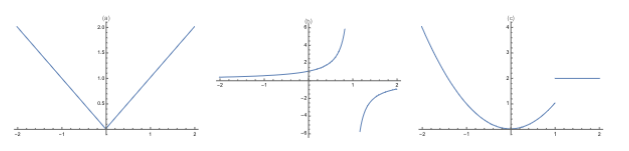
\includegraphics[width=8cm]{./images/continu.png}
	\end{center}
	\caption{a) Continue functie, stukgewijs continue afgeleide (als je afleid krijg je een singulareit) b) Heeft een singulaireit, dus stukgewijs continue, stukgewijs glad continue afleidbaar c) Deze is glad stukgewijs continue afleidbaar, is ook stukgewijs continue }
\end{figure}


\subsection{Taylorontwikkeling}
\label{sec:taylor}

We willen zaken gaan benaderen. Hiervoor gebruiken we:

$ f(x) = f(a) + f'(a)(x-a) + \frac{f''(a)}{2!}(x-a)^2 + \frac{f'''(a)}{3!}(x-a)^3 + ... $

waarbij $a$ het \textbf{werkpunt} is.

Veel voorkomende Taylorontwikkelingen:

See Figure \ref{fig:veel_voorkomend_taylor}.

\begin{figure}[htbp!]
	\centering
	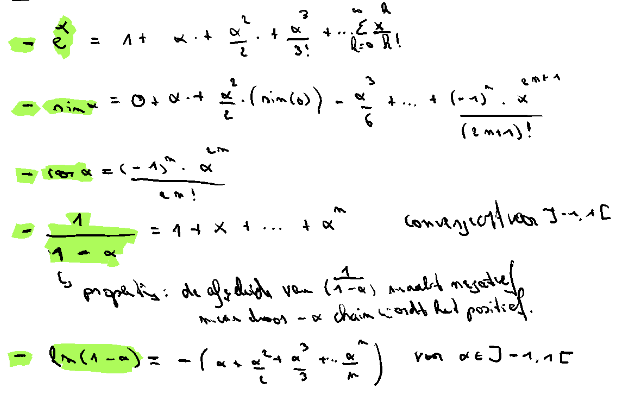
\includegraphics[width=0.8\textwidth]{assets/veel_voorkomend_taylor.png}
	\caption{Simply use the formulas}
	\label{fig:veel_voorkomend_taylor}
\end{figure}

\subsection*{Storingsrekening}

Zie Figuur \ref{fig:storing_solution}.

Of Maple solution \ref{sol:storing}.

\begin{figure}[!htbp]
	\centering
	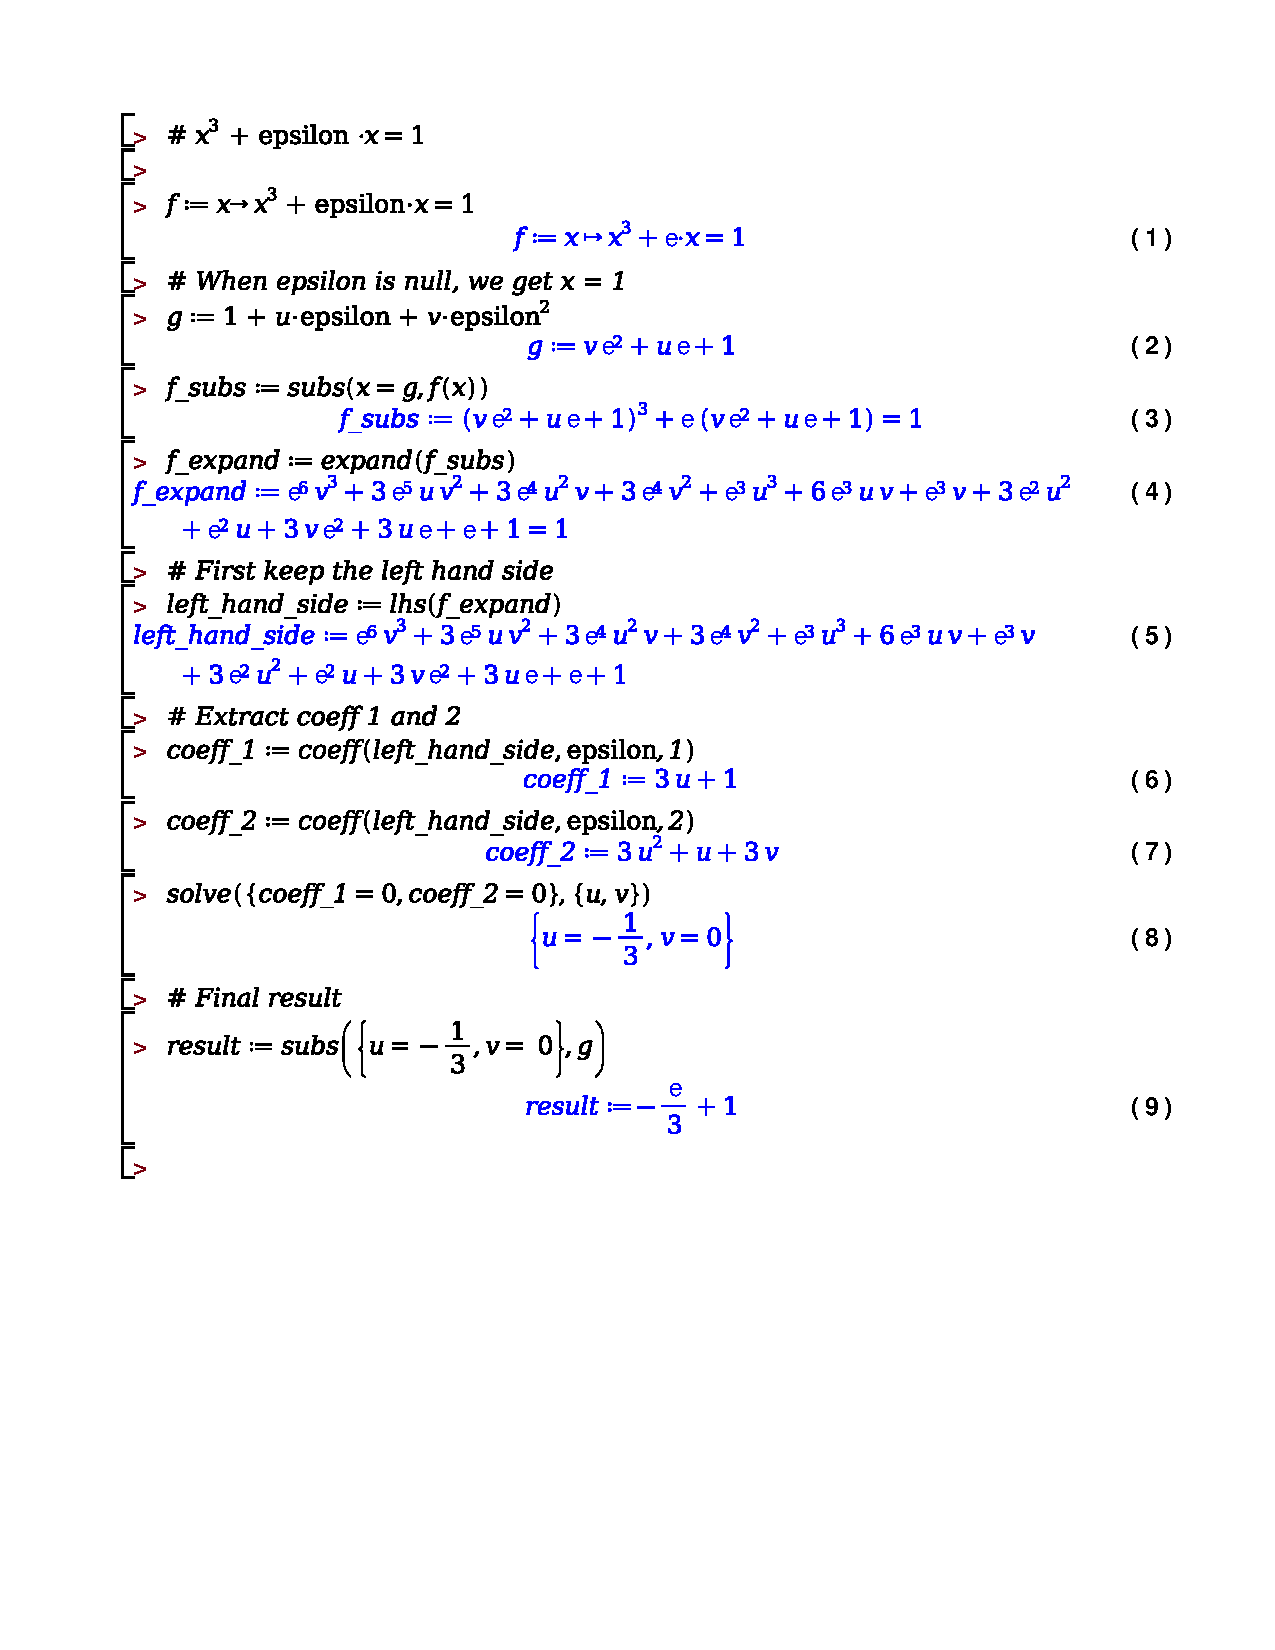
\includegraphics[width=\textwidth]{./storing.pdf}
	\caption{Maple solution}
	\label{sol:storing}
\end{figure}

\begin{figure}[htbp!]
	\centering
	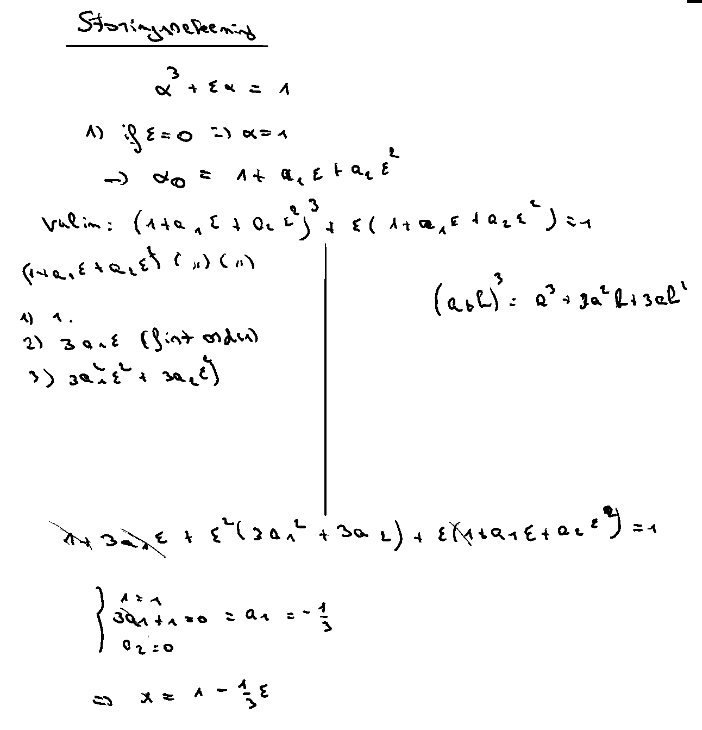
\includegraphics[width=0.8\textwidth]{assets/storing_solution.png}
	\caption{1. Merk op dat als epsilon 0 is, dan is x = 1. Dus we benaderen value 1: $1 + \epsilon . u + \epsilon^2 . v$. Vul dit in the main equation. Gebruik maple om dit op te lossen en vul $u$ en $v$ in $x_1$}
	\label{fig:storing_solution}
\end{figure}

\subsection{Twee eenvoudige differentiaalvergelijkingen}

\subsubsection{Eerste orde differentiaalvergelijking}

$y'(x) = \lambda y(x)$

Als we dit uitwerken krijgen we:

$ln(y(x)) = \lambda x + C$

$y(x) = e^{\lambda x + C} = e^C e^{\lambda x} = C e^{\lambda x}$ met $C = y(0)$

$y(x) = y(0) e^{\lambda x}$

\subsubsection*{Radioactief verval}

Zie Figuur \ref{fig:radio_solution}.

\begin{figure}[htbp!]
	\centering
	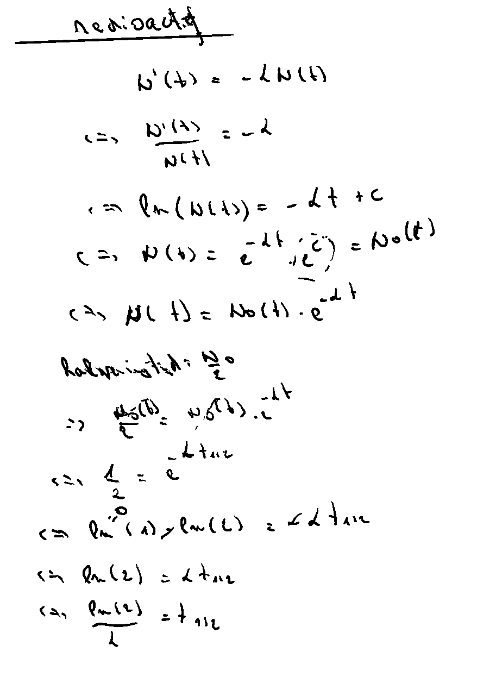
\includegraphics[width=0.8\textwidth]{assets/radio_solution.png}
	\caption{Vindt eerst de differentiaalvergelijking (zie eerste differentiaalvergelijking). Dan kunnen we de oplossing gelijkstellen aan $N_0 / 2$. Werk dit uit en je hebt $t_{1/2}$ gevonden}
	\label{fig:radio_solution}
\end{figure}

\subsubsection{Tweede orde differentiaalvergelijking}

$y''(x) = \lambda y(x)$

Hierbij heb je 3 gevallen:

1. $\lambda > 0$: $y(t) = A e^{\sqrt{\lambda} t} + B e^{-\sqrt{\lambda} t}$

2. $\lambda = 0$: $y(t) = A + Bt$

3. $\lambda < 0$: $y(t) = A cos(\sqrt{-\lambda} t) + B sin(\sqrt{-\lambda} t)$

\subsubsection{Complexe getallen}

Algemene vorm: $z = a + bi$

waarbij $a$ reeel, $b$ imaginair en $i^2 = -1$

\textbf{inverse}: $(a + bi)^{-1} = \frac{a - bi}{a^2 + b^2}$

\textbf{complement}: $z = a + bi \rightarrow z^* = a - bi$

\textbf{modulus}: $|z| = \sqrt{a^2 + b^2}$

in \textbf{polaire vorm}:

$e^{i\theta} = cos(\theta) + i sin(\theta)$ (Dit kan via Taylor bewezen worden (zie oefeningen))

Okey, nu nog een paar goniometrische formules:

$sin^2(x) + cos^2(x) = 1$

$sin(x) = \frac{e^{ix} - e^{-ix}}{2i}$

$sin(2x) = 2sin(x)cos(x)$

$cos(x) = \frac{e^{ix} + e^{-ix}}{2}$

$cos(2x) = cos^2(x) - sin^2(x)$

\subsubsection{Hoofdstelling van de algebra}

Als we een kwadratisch veelterm hebben: $ax^2 + bx + c = 0$

Dan vinden we de nulpunten (oplossingen) met:

$x_1 = \frac{-b + \sqrt{b^2 - 4ac}}{2a}$

$x_2 = \frac{-b - \sqrt{b^2 - 4ac}}{2a}$

met $b = -4*a*c$ vinden we de discriminant.

\section{Lineare Algebra}

\subsection{Lineare onafhanlijkheid}

\textbf{Lineare onafhankelijkheid} betekent dat de vectoren niet op een lijn liggen. Dit betekent dat de determinant van de matrix niet 0 is.
Maar ook dat de vectoren niet een lineaire combinatie van elkaar zijn.

\begin{figure}[htbp!]
	\centering
	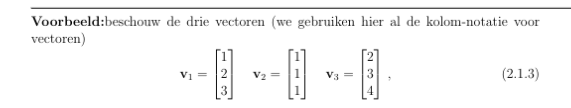
\includegraphics[width=0.8\textwidth]{images/ex_lin_on.png}
	\caption{1. Merk op dat als epsilon 0 is, dan is x = 1. Dus we benaderen value 1: $1 + \epsilon . u + \epsilon^2 . v$. Vul dit in the main equation. Gebruik maple om dit op te lossen en vul $u$ en $v$ in $x_1$}
\end{figure}

$v_1, v_2, v_3$ zijn lineair onafhankelijk. Maar $v_1$ en $v_2$ bijvoorbeeld, vormen een lineaire combinatie van $v_3$

\subsection{Inproduct, Norm, Orthogonaliteit}

- \textbf{Inproduct}: $u \dot v = \sum_{i=1}^{n} u_i v_i$

- \textbf{Norm}: $||v|| = \sqrt{v \dot v}$

Side note: om de \textbf{hoek} tussen 2 vectoren te vinden, $\frac{u\dot v}{||u|| ||v||} = cos(\theta)$

\subsection{Gramm-Schmidt}

Dit gaat ons toelaten om een basis te vinden van vectoren.

$v_1$ = $u_1$/ $||u_1||$

$v_2$ = $u_2 - \frac{u_2 \dot v_1}{Norm} v_1$

$v_x$ = ...

Ook definieerd het dat een vector $v = v^{||} + v^{\perp}$

Waarbij $v^{||}$ de projectie is van $v$ op $u$ en $v^{\perp}$ de projectie op de orthogonale basis.

$v^{||} = (u_1 \dot y) u_1 + (u_2 \dot y) u_2 + ...$

\subsubsection{Voorbeeld Gramm-Schmidt}

Zie Figuur \ref{fig:gramm_schmidt}.


\begin{figure}[htbp!]
	\centering
	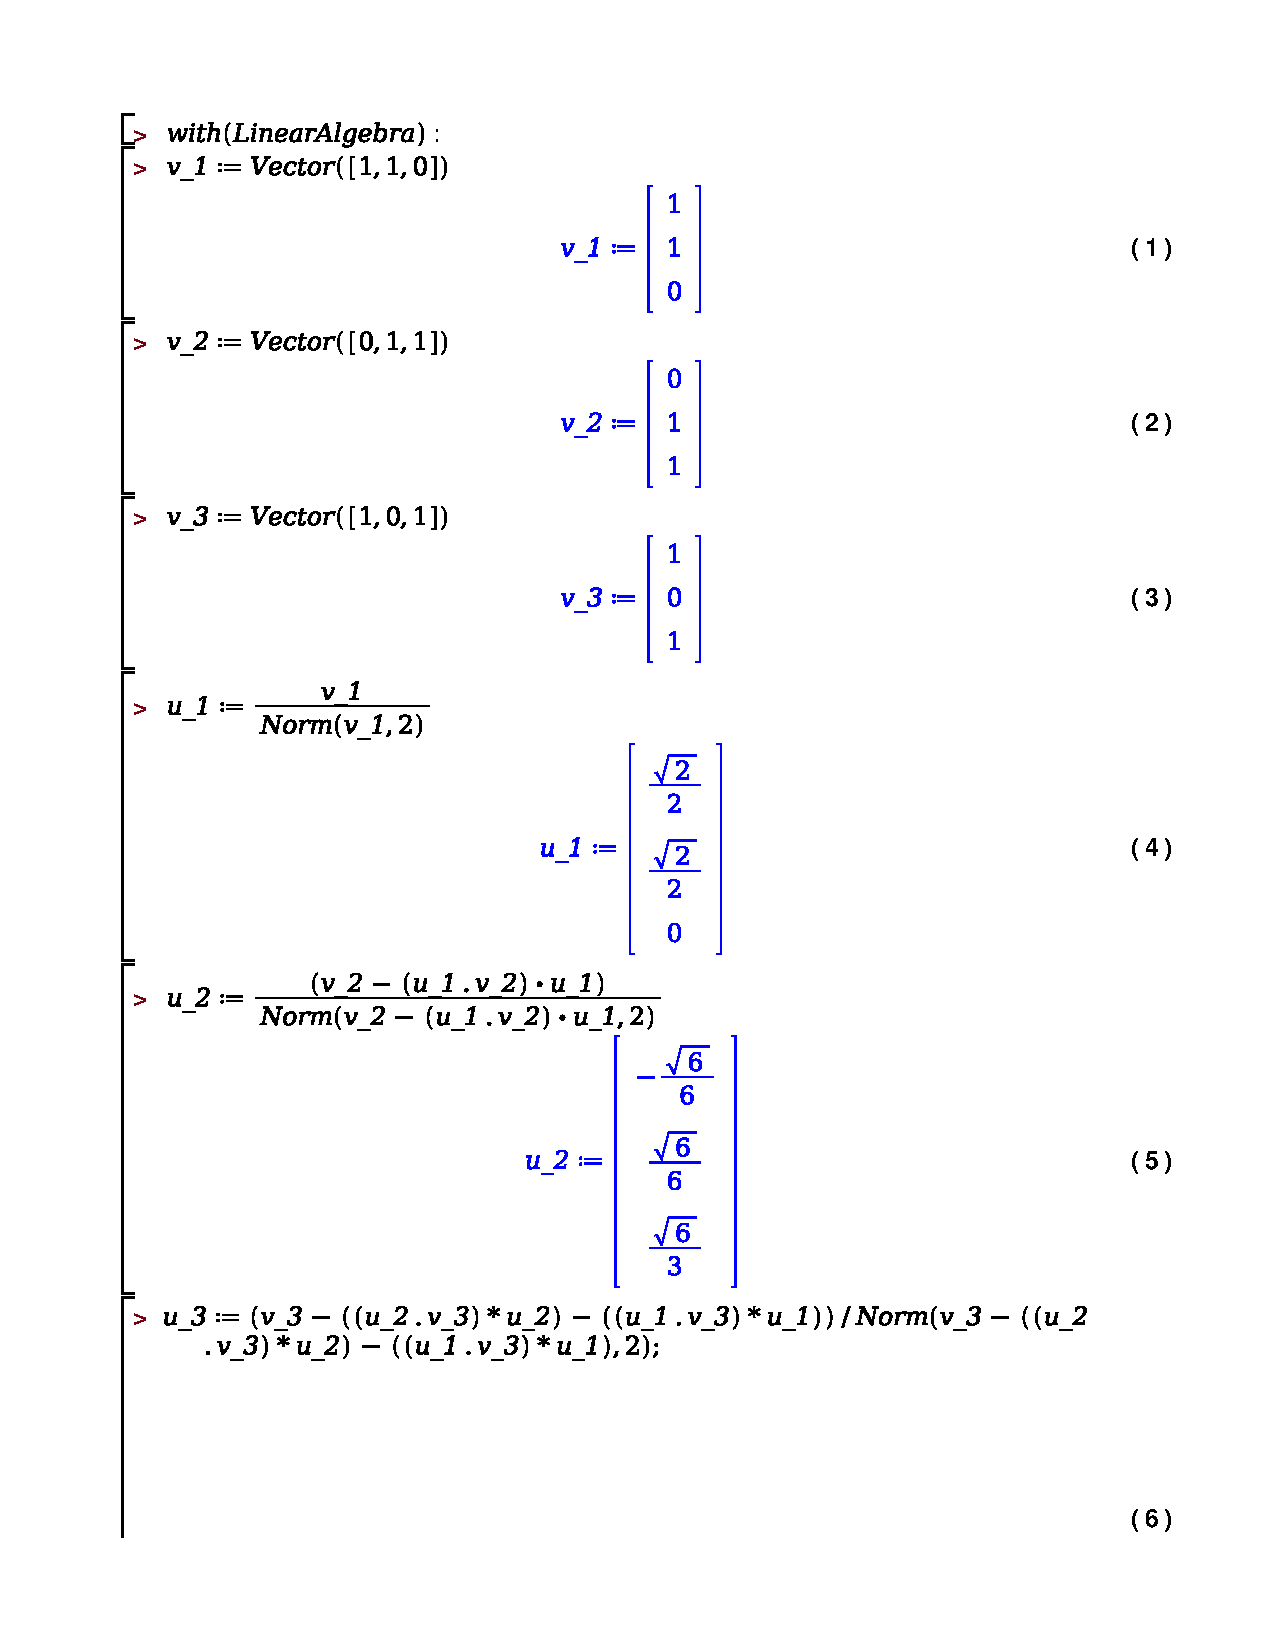
\includegraphics[width=0.8\textwidth]{./gram.pdf}
	\caption{Hier gebruiken we dus de iteratieve formule om de basis te vinden.}
	\label{fig:gramm_schmidt}
\end{figure}

\textbf{Note}: Dit kan uitgebreid worden naar functieruimtes. Hiervoor gaan we een oefening zien in het werkcollege.

\subsection{Matrices}

Typische vorm: $y=Ax$

Het \textbf{getransponeerde} is $A^T$, de rijen worden kolommen en omgekeerd.

Hier geldt dan dat: $(AB)^T = B^T A^T$, dus je draait de matrices om

\subsection{Kolomruimte, rijruimte, nulruimte}

- \textbf{Kolomruimte}: alle mogelijke lineaire combinaties van de kolommen ( $K(A)$)

- \textbf{Rijruimte}: alle mogelijke lineaire combinaties van de rijen ($K(A^T)$)

- \textbf{Nulruimte}: alle vectoren die op 0 worden afgebeeld ($N(A)$ of $N(A^T)$)

Zeer belangrijk is dat:

$N(A)$ complementair is aan $K(A^T)$ en $N(A^T)$ is complementair aan $K(A)$

Bij de representatie van het vlak heb je een \textbf{rang}. Dit is basically de hoeveelheid kolommen van $Q$ niet nul zijn.

\subsubsection{Voorbeeld definities}

Zie Figuur \ref{fig:kolom_rij_null}.

\begin{figure}[hbpt!]
	\centering
	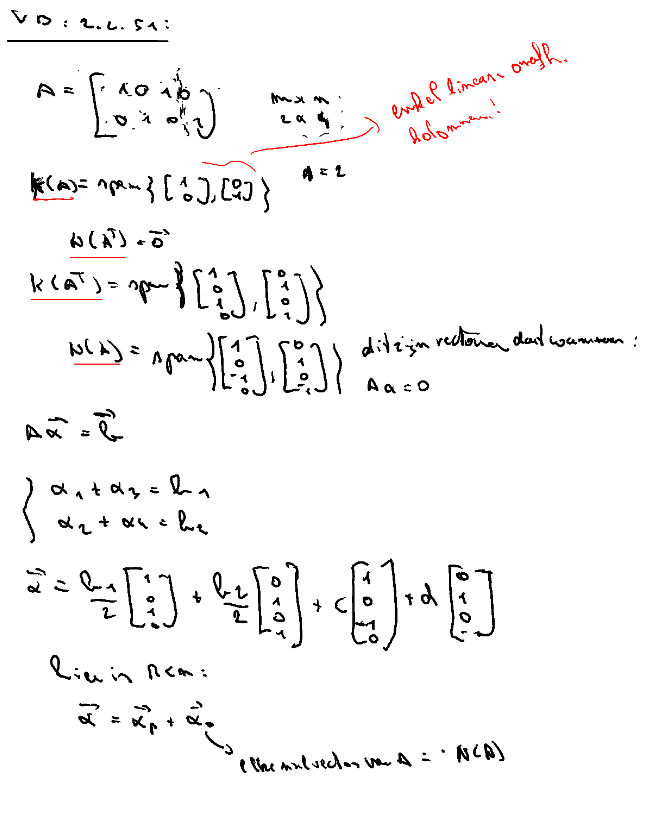
\includegraphics[width=0.8\textwidth]{assets/kolom_rij_null.png}
	\caption{}
	\label{fig:kolom_rij_null}
\end{figure}

\subsection{Matrix Inverse}

$x = A^{-1} y$

Typisch gezien is dit gedaan via: $\frac{1}{det(A)} adj(A)$

Wat heel nuttig is is dat $A A^{-1} = I$ en $A^{-1} A = I$. Dit kan heel wat schrijfwerk vermijden

Weer zoals bij transponeren geldt dat $(AB)^{-1} = B^{-1} A^{-1}$

\subsection{Projectie en kleinste kwadraten benadering}

Zoals we eerder hebben gezien bij Gramm-Schmidt, kunnen we $v= v^{||} + v^{\perp}$ schrijven.

We kunnen er iets abstracter boven plakken en werken met een \textbf{Projector}.

Deze is gedefinieerd als: $P = A (A^T A)^{-1} A^T$ (deze vorm is niet al te belangrijk).

Met de nieuwe definitie $P$ kunnen we nu zeggen dat $v = Pv + (I - P)v$

The following properties hold:

\begin{enumerate}
	\item $P^2 = P$
	\item $P^T = P$
\end{enumerate}

\subsubsection{Voorbeeld Projectie}

Zie Figuur \ref{fig:projectie}.

\begin{figure}
	\begin{center}
		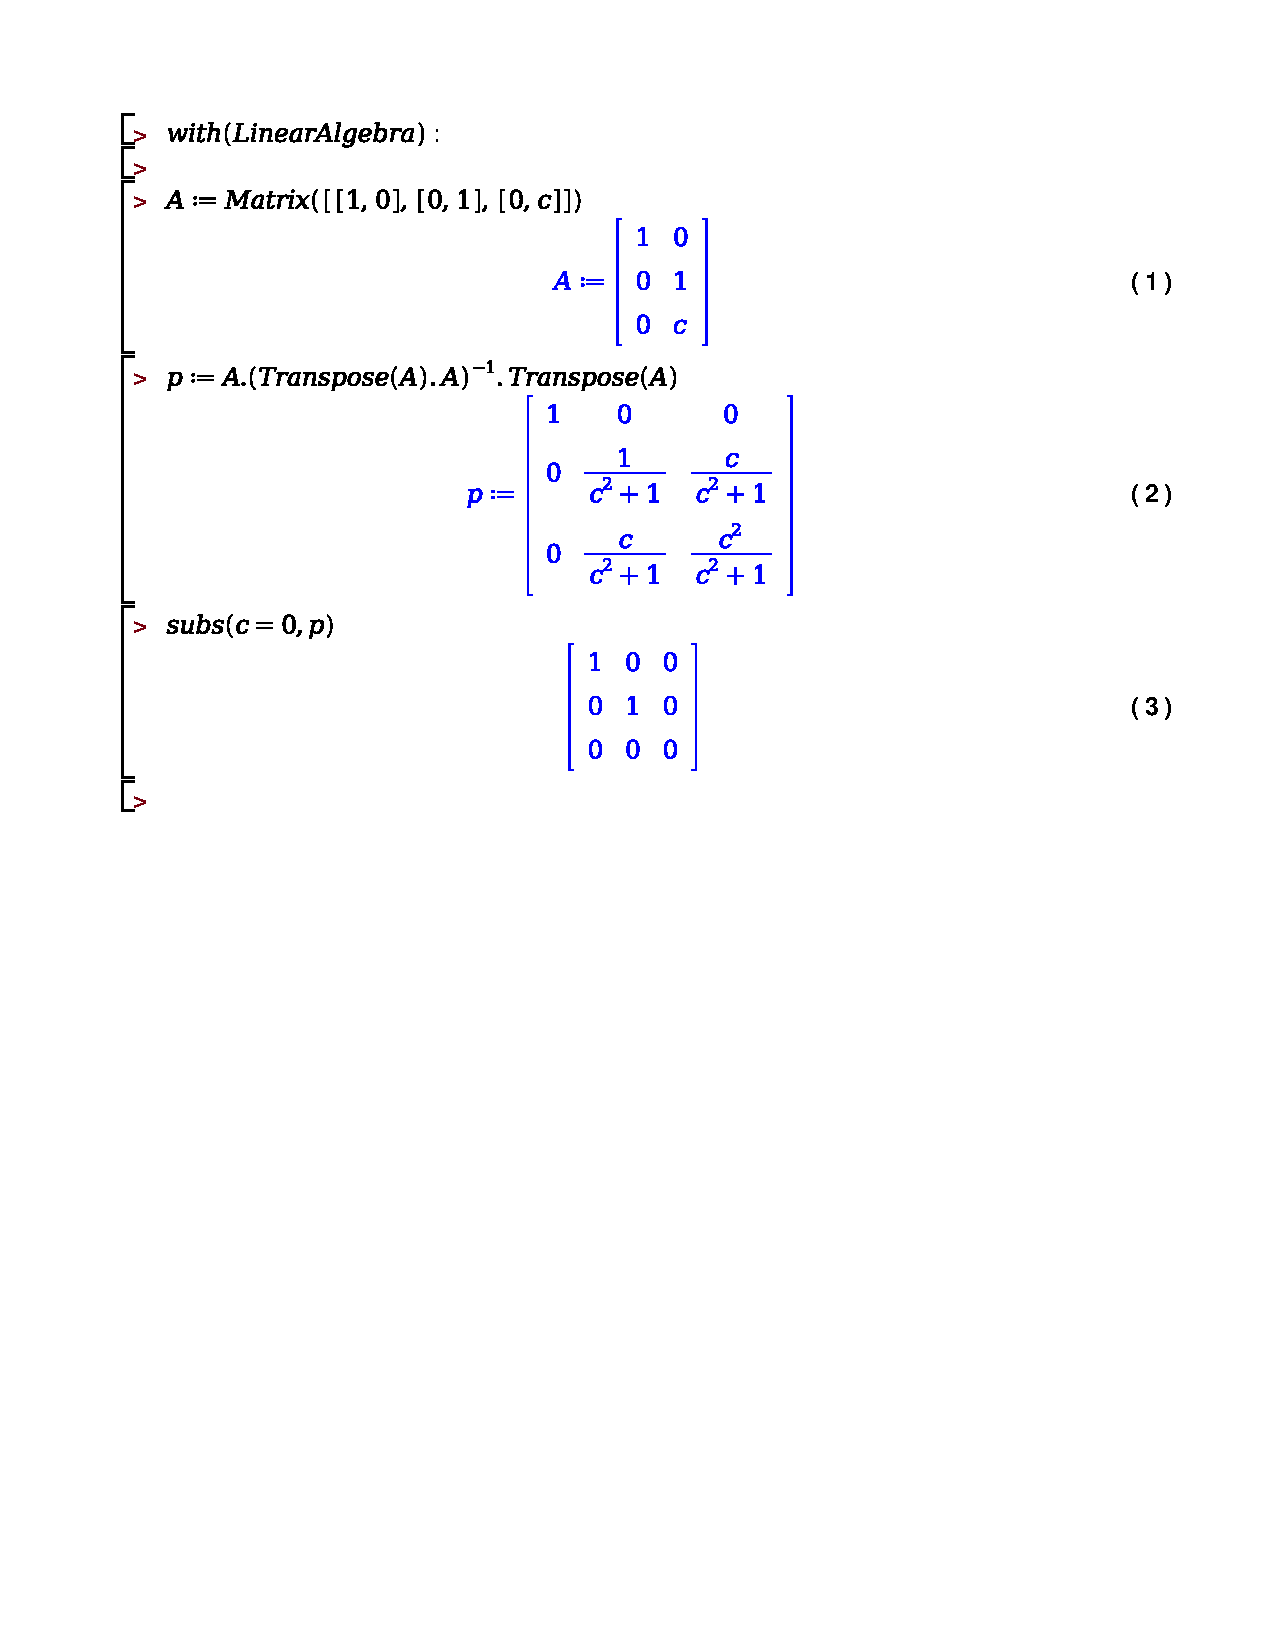
\includegraphics[width=0.95\textwidth]{./projector.pdf}
	\end{center}
	\caption{}\label{fig:projectie}
\end{figure}

\subsection{Kleinste kwadraten fit}

$x = (A^T A)^{-1} A^T y$

Dit gaat ons toelaten om te fitten op data.

In Maple wordt dit gedaan via \texttt{LinearAlgebra:-LeastSquares}.

\subsection{Vierkante matrices}

\subsubsection{Determinant}

De determinant is super handig. Hoe calculeren we deze?

Let \(\mathbf{A}\) be a \(3 \times 3\) matrix:
\[
	\mathbf{A} =
	\begin{pmatrix}
		a_{11} & a_{12} & a_{13} \\
		a_{21} & a_{22} & a_{23} \\
		a_{31} & a_{32} & a_{33}
	\end{pmatrix}
\]

The determinant of \(\mathbf{A}\), denoted as \(\det(\mathbf{A})\) or \(|\mathbf{A}|\), is calculated as:
\[
	\det(\mathbf{A}) = a_{11}(a_{22}a_{33} - a_{23}a_{32}) - a_{12}(a_{21}a_{33} - a_{23}a_{31}) + a_{13}(a_{21}a_{32} - a_{22}a_{31})
\]

Expanding the terms, we have:
\[
	\det(\mathbf{A}) = a_{11}a_{22}a_{33} - a_{11}a_{23}a_{32} - a_{12}a_{21}a_{33} + a_{12}a_{23}a_{31} + a_{13}a_{21}a_{32} - a_{13}a_{22}a_{31}
\]

Properties:

\begin{enumerate}
	\item $det(A) = det(A^T)$
	\item $det(AB) = det(A) det(B)$
	\item $det(A) = 0 -> linear dependent$
\end{enumerate}

\subsection{Basic rotation matrix}

$R(\theta) = \begin{bmatrix} cos(\theta) & -sin(\theta) \\ sin(\theta) & cos(\theta) \end{bmatrix}$

So a typical transformation equation looks like:

$\begin{bmatrix} x' \\ y' \end{bmatrix} = \begin{bmatrix} cos(\theta) & -sin(\theta) \\ sin(\theta) & cos(\theta) \end{bmatrix} \begin{bmatrix} x \\ y \end{bmatrix}$
with the middle matrix being **inverse**.

\subsubsection{Example}

See Figure \ref{fig:rotation} and \ref{fig:rotationex}.

\begin{figure}[htbp!]
	\begin{center}
		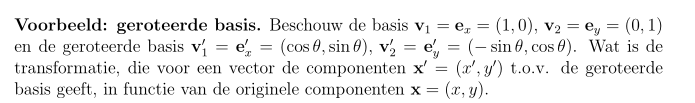
\includegraphics[width=0.7\textwidth]{./images/rotation.png}
	\end{center}
	\caption{Rotation opgave}
	\label{fig:rotation}
\end{figure}

\begin{figure}[htbp!]
	\begin{center}
		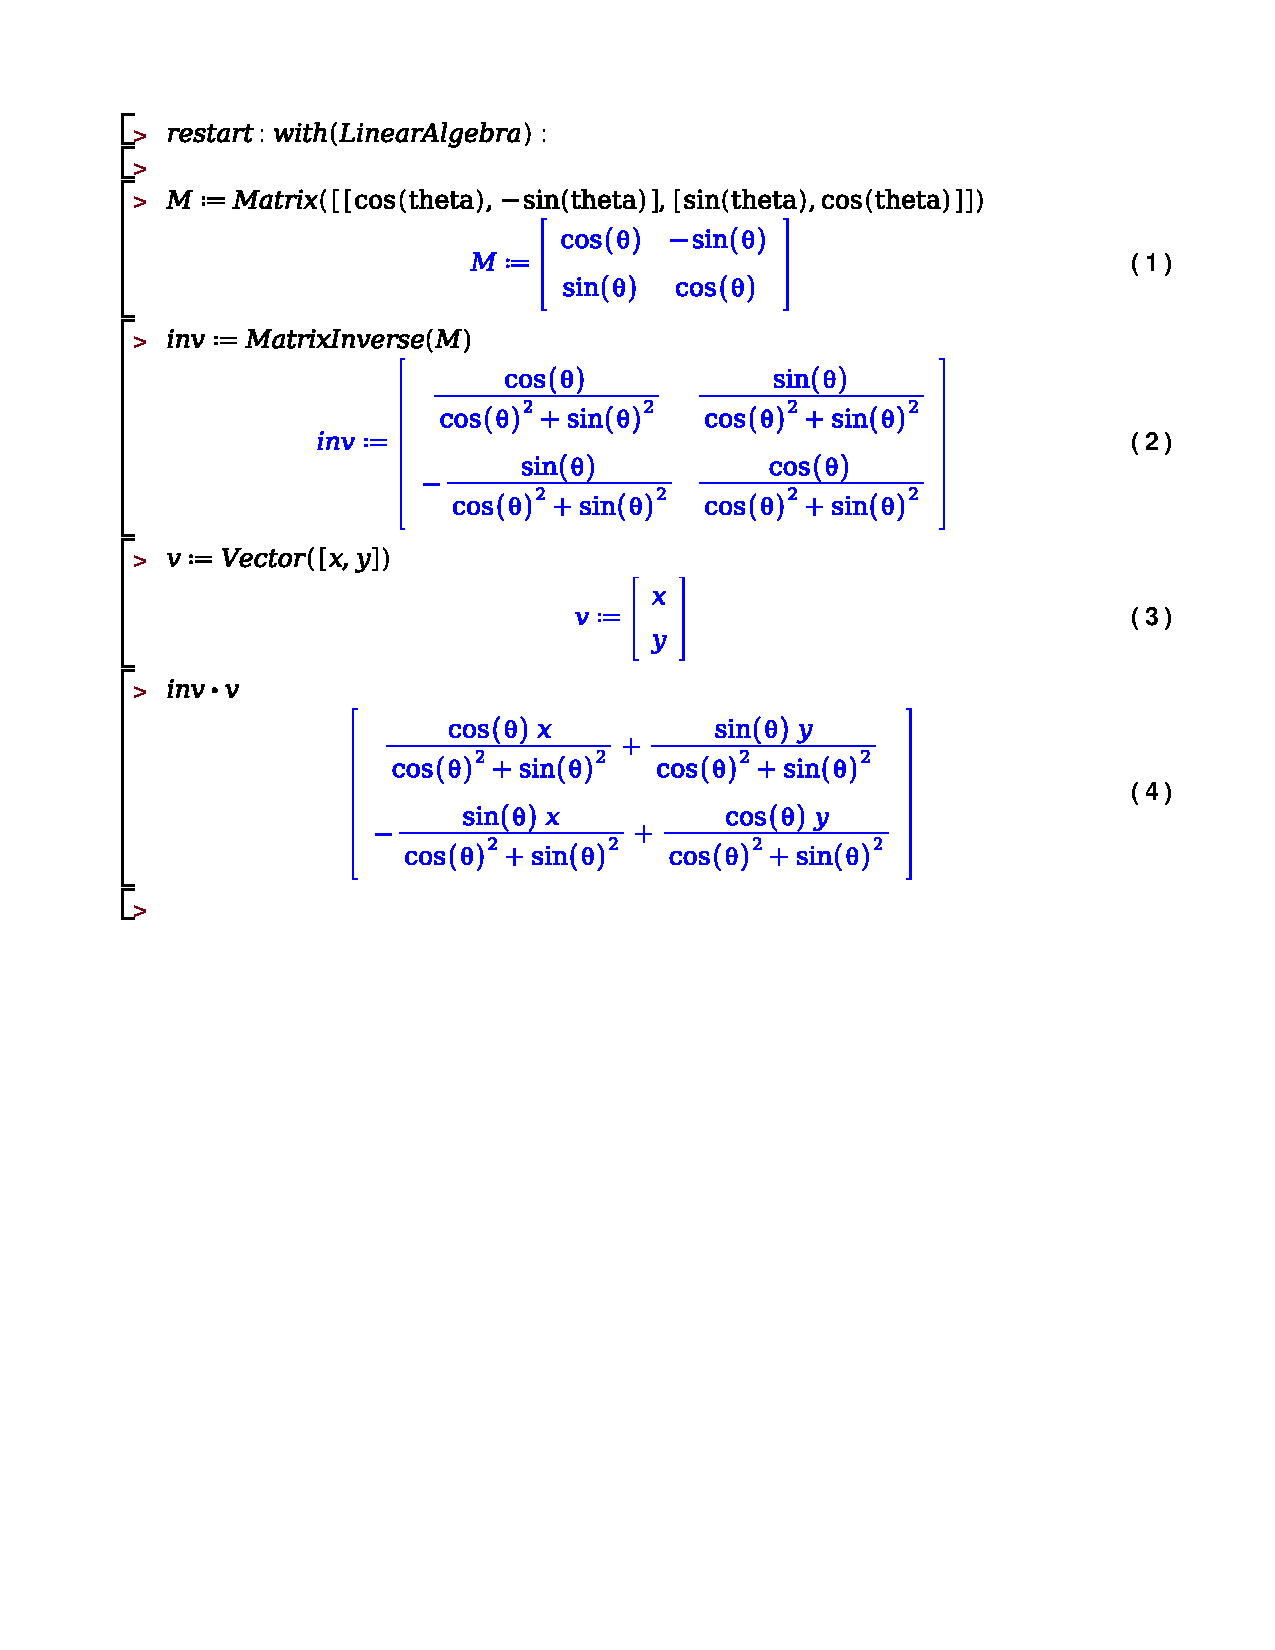
\includegraphics[width=0.7\textwidth]{./rotation.pdf}
	\end{center}
	\caption{Rotation antwoord}
	\label{fig:rotationex}
\end{figure}

\subsection{Eigenvectoren, eigenwaarden, diagonalisatie en de Jordan-decompositie}

$v_i$ is een eigenvector van A als $Av_i = \lambda_i v_i$

$p_A(\lambda) = det(A - \lambda I) = 0$

- geometrische multipliciteit: aantal lineair onafhankelijke eigenvectoren (je moet de eigenvalue invullen en row echelon reduced form verkrijgen. Dan zie je hoeveel eigenvectoren er degelijk zijn)

Figuur \ref{fig:mult} toont een voorbeeld van de multipliciteit.

\begin{figure}[htbp!]
	\begin{center}
		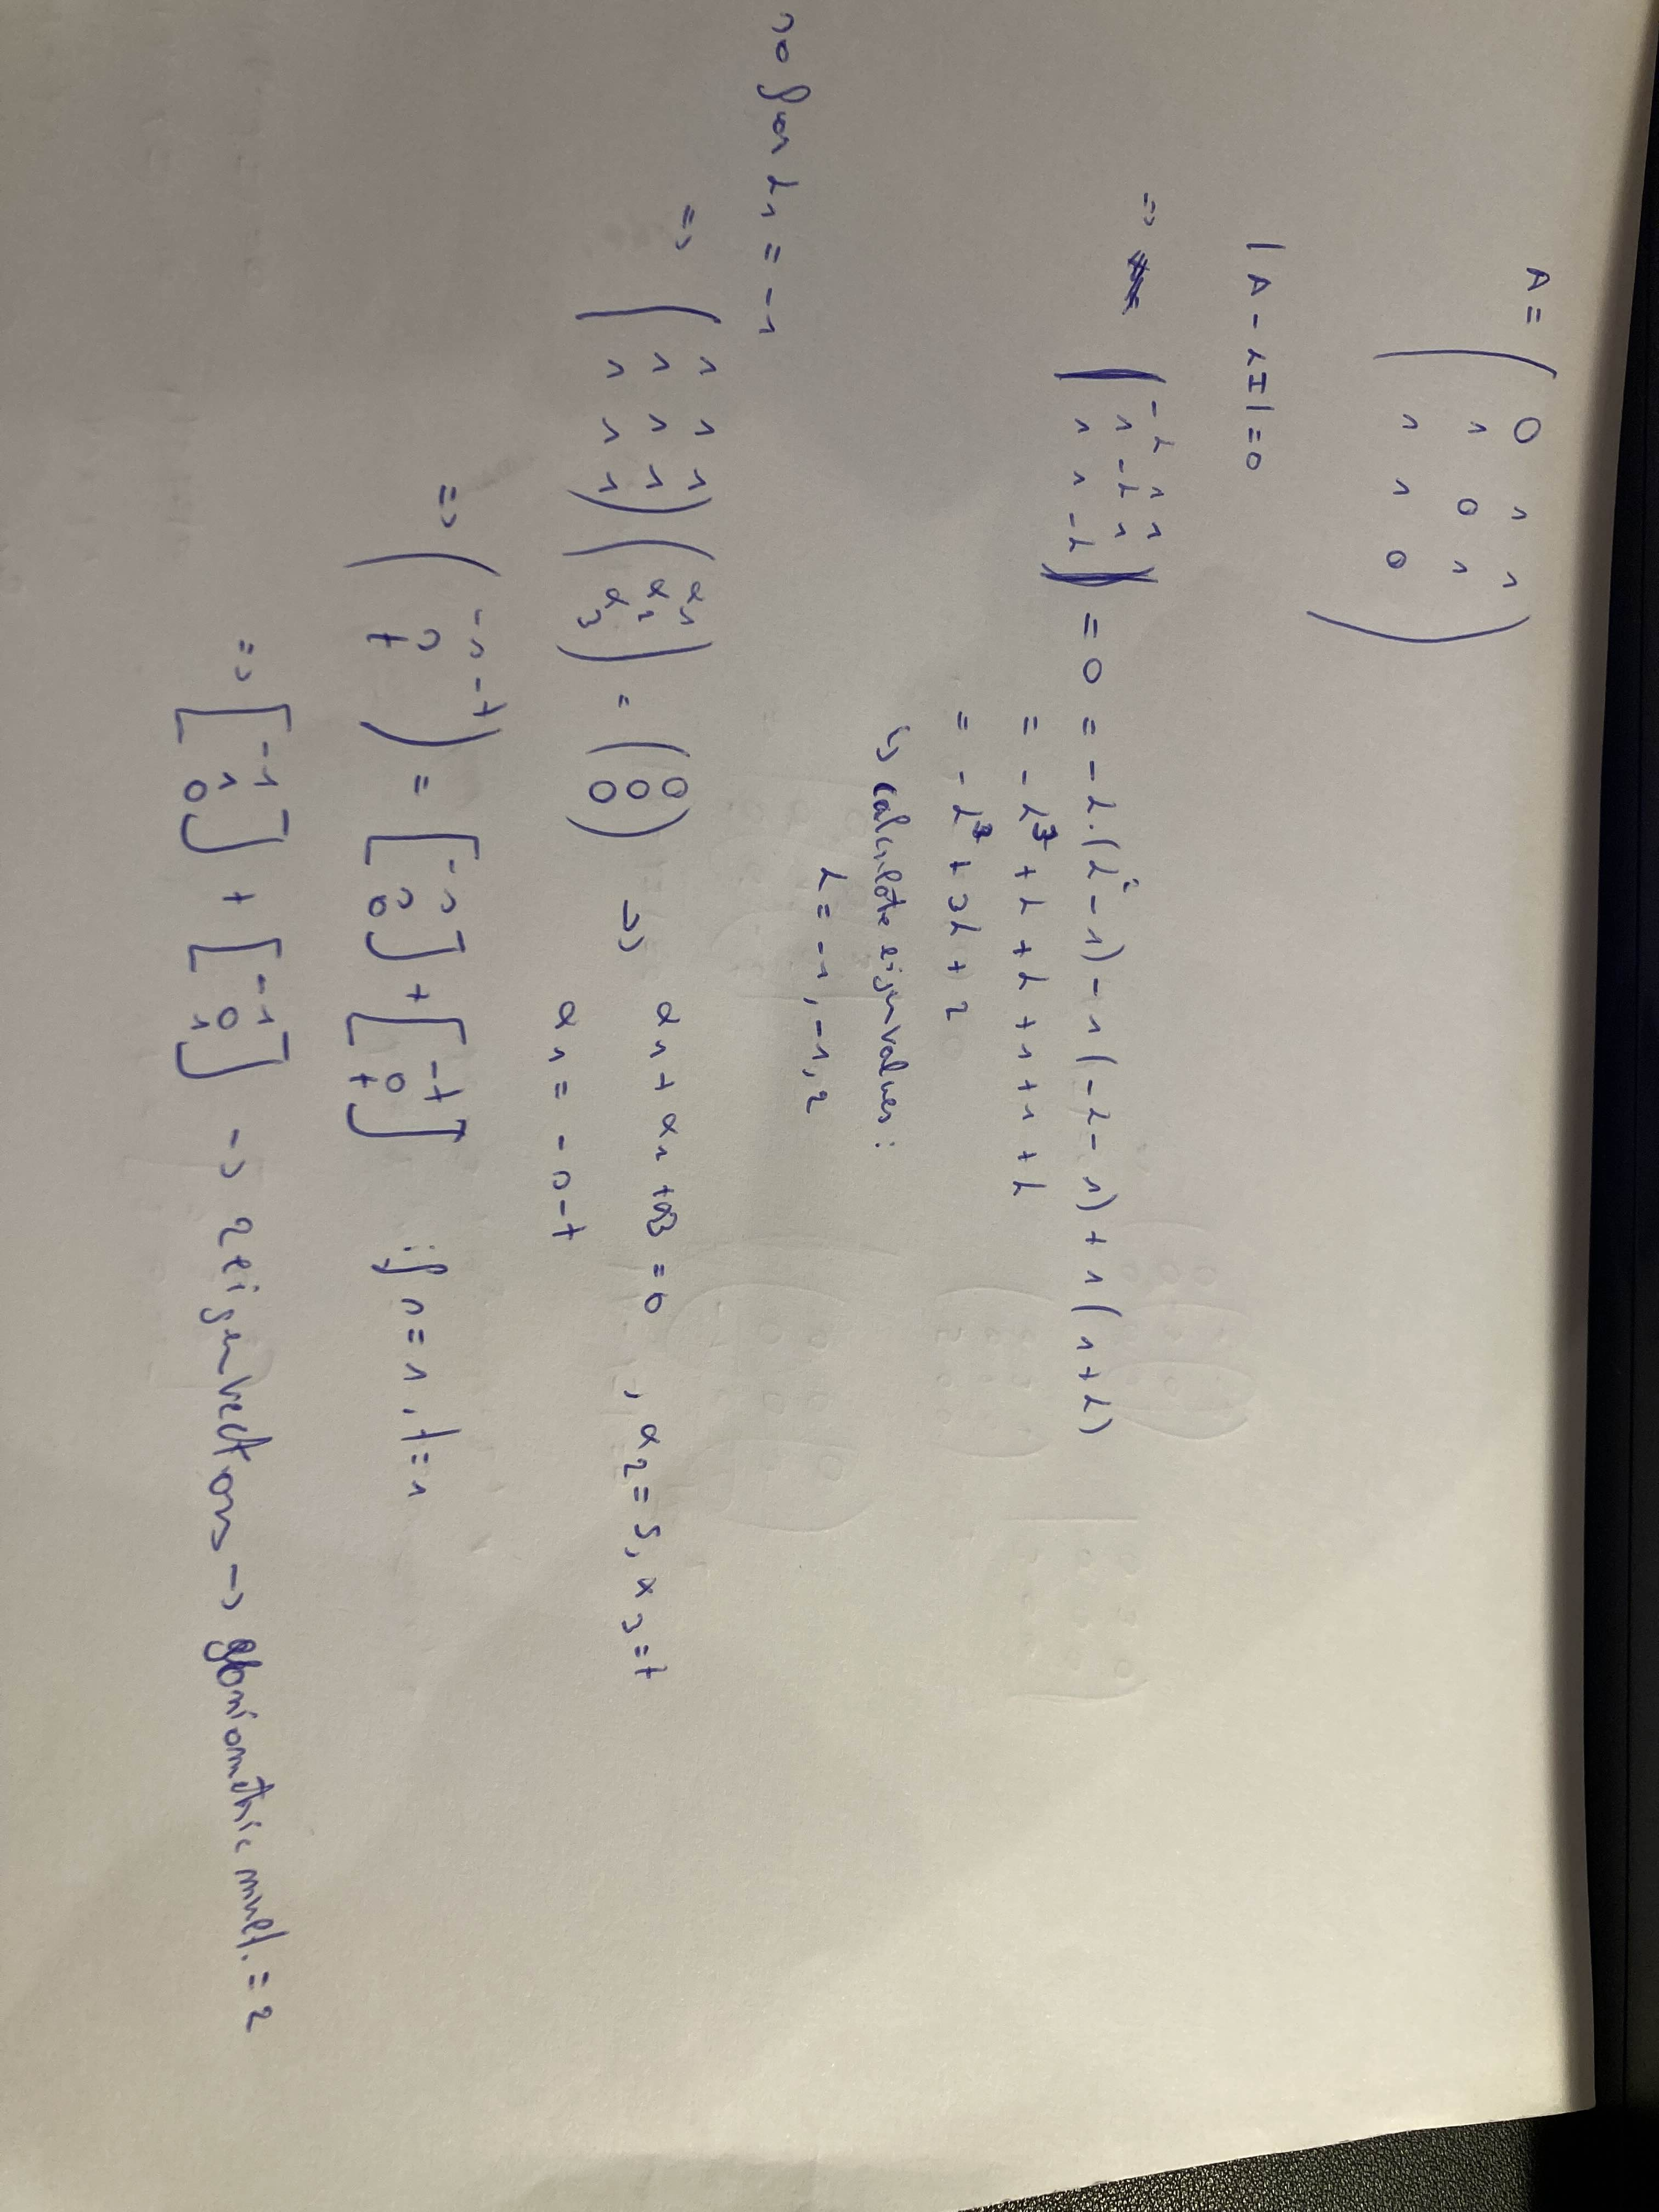
\includegraphics[width=0.95\textwidth]{./images/mult.jpg}
	\end{center}
	\caption{Een voorbeeld van de multipliciteit}
	\label{fig:mult}
\end{figure}

- algebraische multipliciteit: aantal keer dat de eigenwaarde voorkomt in de determinant

Indien alle geometrische multipliciteiten gelijk zijn aan de algebraische multipliciteiten, dan is de matrix diagonaliseerbaar.
$A = MDM^{-1}$

met $D$ een diagonale matrix met de eigenwaarden op de diagonaal.
en $M$ een matrix met de eigenvectoren.

\subsection{Jordan Form}

$A = MJM^{-1}$
met $J$ een Jordan matrix.
Dit is nodig indien de dimensie van de eigenruimte (geometrische multipliciteit) kleiner is dan de algebraische multipliciteit.
Aka, de matrix is niet diagonaliseerbaar. \ref{fig:jordan} \ref{fig:jordan_ex}

\begin{figure}[htbp!]
	\begin{center}
		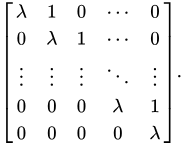
\includegraphics[width=0.95\textwidth]{./images/jordan.png}
	\end{center}
	\caption{Jordan matrix}
	\label{fig:jordan}
\end{figure}

\begin{figure}[htbp!]
	\begin{center}
		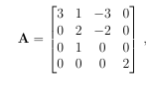
\includegraphics[width=0.95\textwidth]{./images/ex_joran.png}
	\end{center}
	\caption{Jordan matrix example}
	\label{fig:jordan_ex}
\end{figure}

This gives us: \ref{fig:jordan_sol}

\begin{figure}[htbp!]
	\begin{center}
		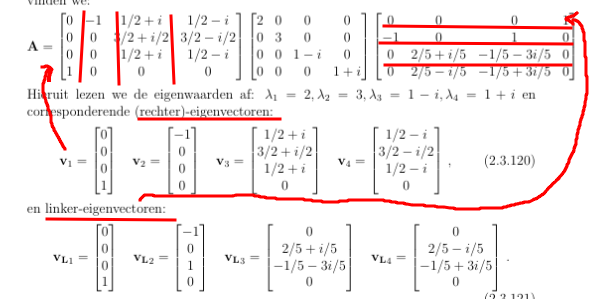
\includegraphics[width=0.95\textwidth]{./images/sol_jordan.png}
	\end{center}
	\caption{Jordan matrix solution}
	\label{fig:jordan_sol}
\end{figure}

\subsubsection{Example}

See Figure \ref{fig:jordan_ex_2}.
\begin{figure}[htbp!]
	\begin{center}
		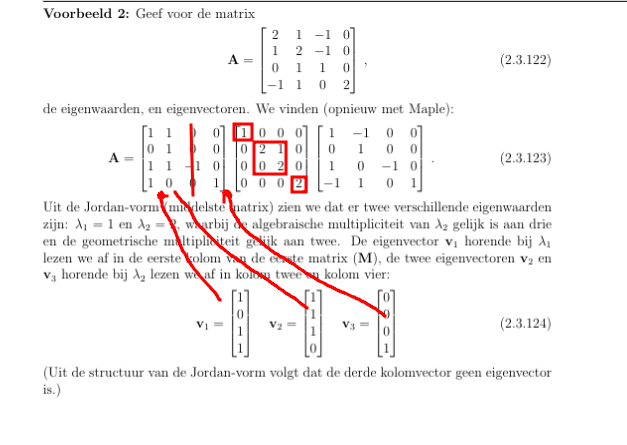
\includegraphics[width=0.95\textwidth]{./images/jordan_ex_2.png}
	\end{center}
	\caption{Jordan matrix example 2}
	\label{fig:jordan_ex_2}
\end{figure}

\subsection{Matrixmachten en iteratieve matrixvergelijkingen}

$A^k = M D^k M^{-1}$ voor diagonaliseerbare matrices

$A^k = M J^k M^{-1}$ voor niet-diagonaliseerbare matrices

met diagonaal matrix: \ref{fig:diag}

\begin{figure}[htbp!]
	\begin{center}
		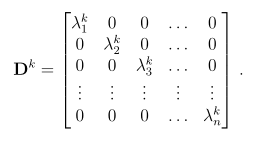
\includegraphics[width=0.95\textwidth]{./images/diag.png}
	\end{center}
	\caption{Diagonaal matrix}
	\label{fig:diag}
\end{figure}

\textbf{iteratieve matrixvergelijking}: $x_k = M D^k M^{-1} x_0$ Op deze manier kun je telkens de $k_{de}$ stap berekenen.

Dit is enkel voor de diagonaliseerbare matrices. ($A^k = M D^k M^{-1}$)

\textbf{asymptotisch gedrag}: $\lim_{k \to \infty} u_k = \lambda^k (v_{L1} * u_0) v_1$

$v_1$ is een fixed point in het asymptotisch gedrag.

\subsubsection{Voorbeeld}

Zie Figuur \ref{fig:fibo}.

\begin{figure}[htbp!]
	\begin{center}
		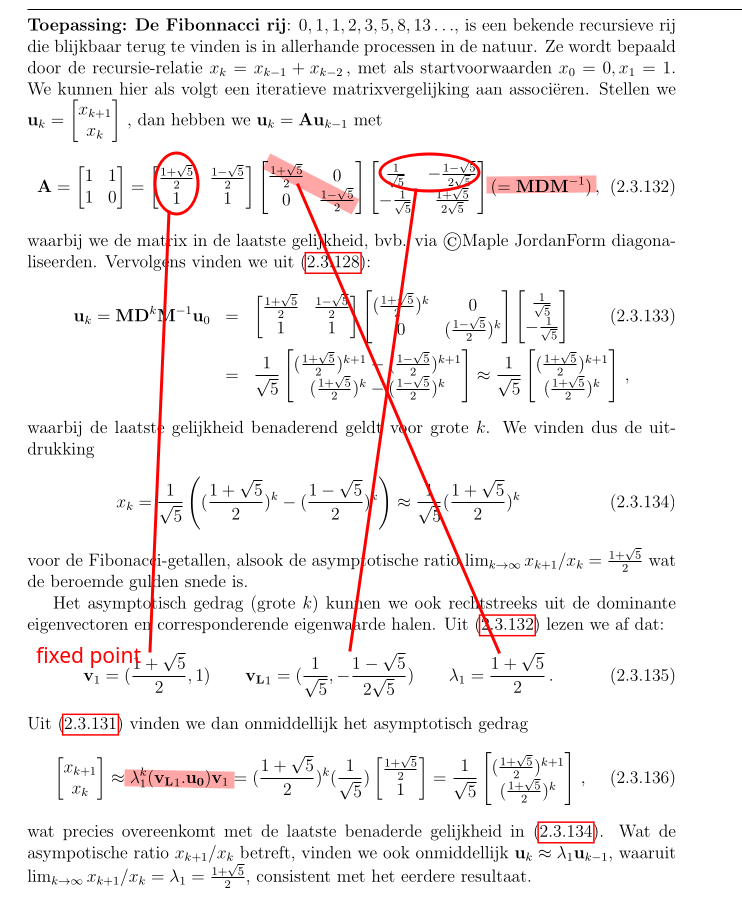
\includegraphics[width=0.95\textwidth]{./images/fibo.png}
	\end{center}
	\caption{Fibonacci voorbeeld}
	\label{fig:fibo}
\end{figure}

In het bovenstaande zien we dat $\lambda_1$ de dominante eigenwaarde is. Daardoor kunnen we de fixed point berekenen met:

$\lambda_1^k (v_{L1} . u_0) v_1$

Omdat $\lambda_1$ dominant is, nemen we voor $v_1$ de eerste kolom van $M$ en voor $v_{L1}$ de eerste rij van $M^{-1}$

Dit kan toegepast worden in de zogezegde \textbf{Markov proces}

algemene vorm: $u_k = P u_{k - 1}$
waarbij $P$ een matrix is die de overgangen tussen de verschillende states aangeeft met probabiliteit.
$\sum p_{ij} = 1$

Ook goed om te weten is dat wanneer de matrix strikt positieve getallen heeft, dat matrix $P$ een uniek dominante eigenwaarde $\lambda_1 = 1$ heeft met $v_1$ een positieve eigenvector. Deze $v_1$ is dan ook een fixed point.

\subsubsection{Voorbeeld Markov proces}

Zie Figuur \ref{fig:markov} and \ref{fig:markovsol}.

\begin{figure}[htbp!]
	\begin{center}
		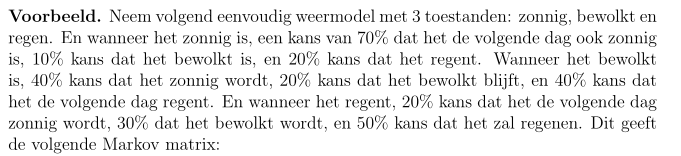
\includegraphics[width=0.95\textwidth]{./images/markov.png}
	\end{center}
	\caption{Markov proces}
	\label{fig:markov}

\end{figure}
\begin{figure}[htbp!]
	\begin{center}
		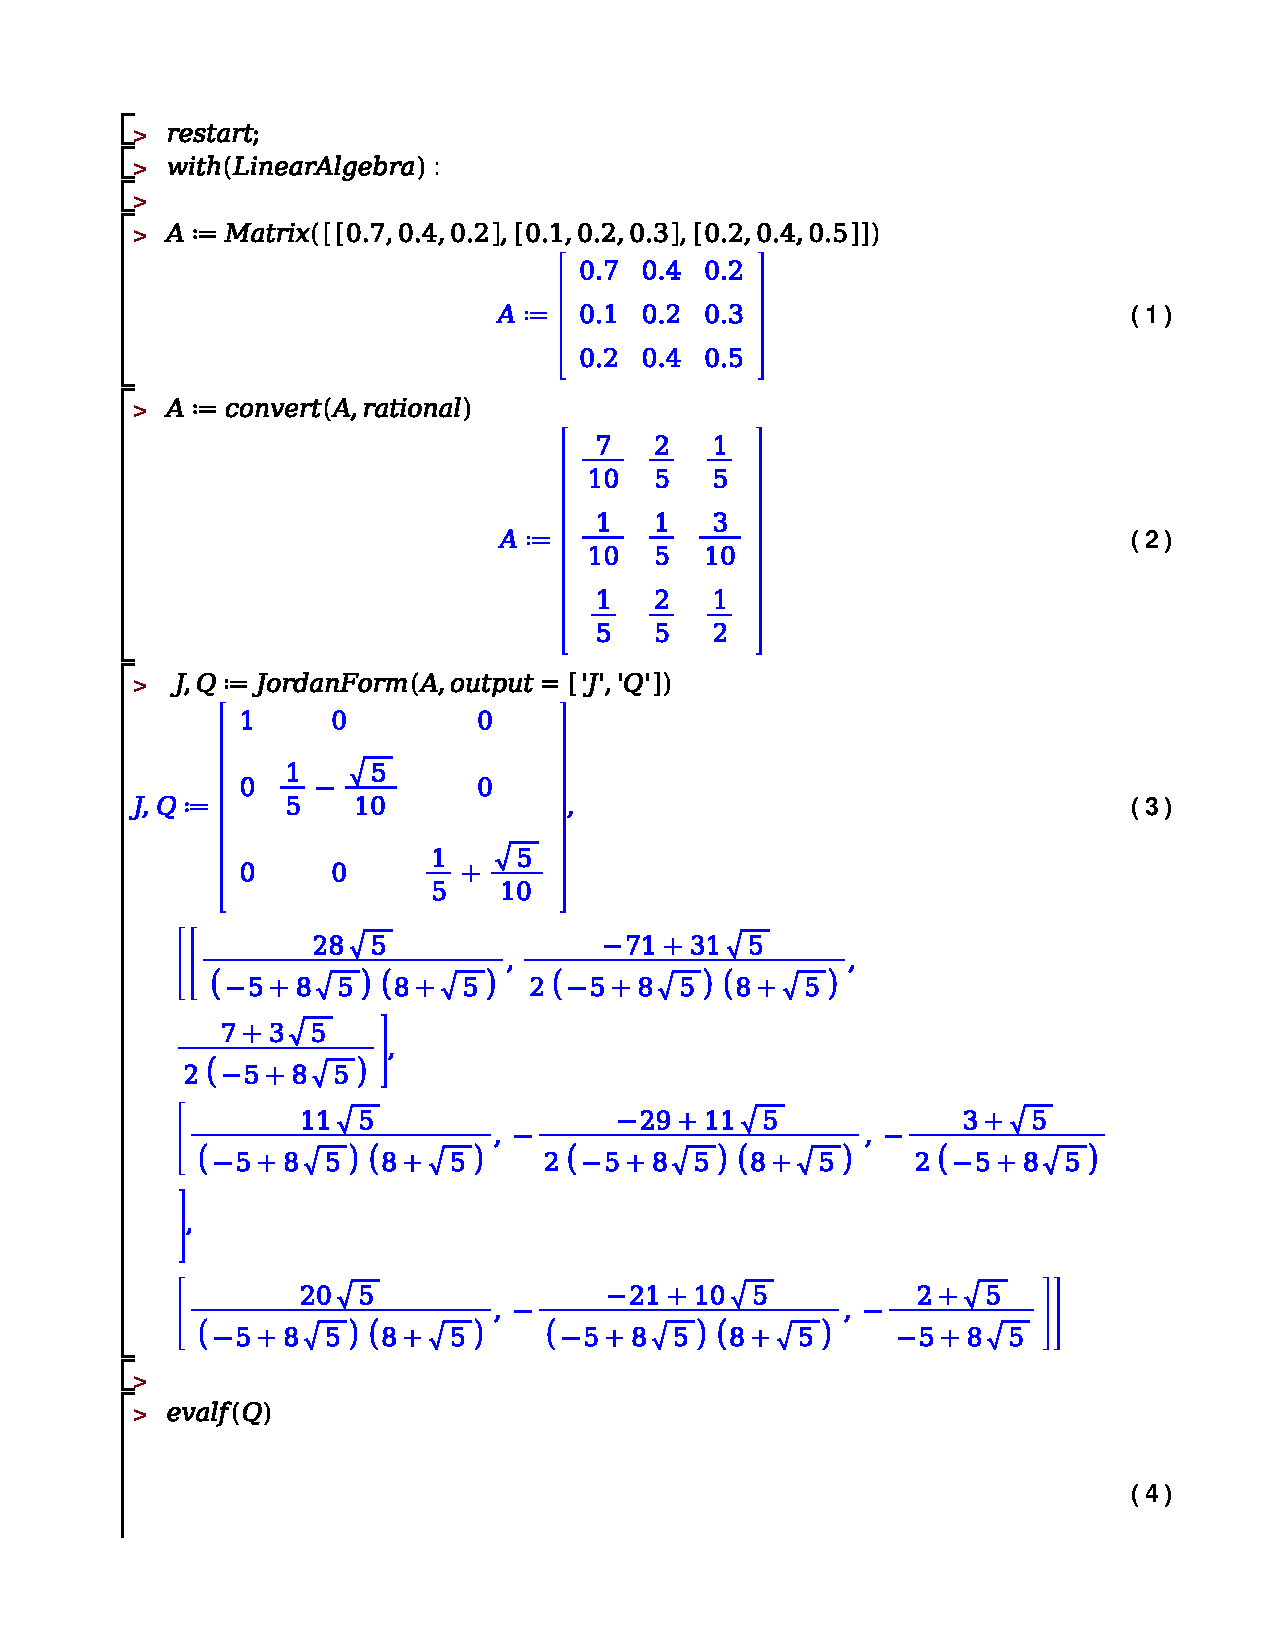
\includegraphics[width=0.95\textwidth]{./markov.pdf}
	\end{center}
	\caption{Markov proces solution}
	\label{fig:markovsol}
\end{figure}

\subsection{Matrixexponent en lineaire differentiaalvergelijkingen}

Hier gaan we een matrix plaatsen de exponent.

$e^{At} = M e^{Dt} M^{-1}$ -> concreet voorbeeld

\textbf{Algemeen}:

$e^{A} = \sum_{k=0}^{\infty} \frac{A^k}{k!}$

of

$e^{A} = M e^{D} M^{-1}$ || $e^{A} = M e^{J} M^{-1}$ (niet-diagonaliseerbare matrices)

In matrix vorm zie je het volgende: \ref{fig:matrix_expo}

\begin{figure}[htbp!]
	\begin{center}
		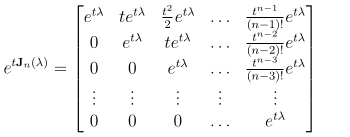
\includegraphics[width=0.95\textwidth]{./images/matrix_expo.png}
	\end{center}
	\caption{Matrix exponent}
	\label{fig:matrix_expo}
\end{figure}

Note: Maple geeft de functie `MatrixExponential(A, t)` om $e^{At}$ te berekenen.

\subsubsection{eerste-orde differentiaalvergelijking}

$y'(t) = Ay(t)$

$y(t) = e^{At} y(0)$

\subsubsection{n-de differentiaalvergelijkin}

Hetzelfde als hierboven

\subsubsection{Herschrijf de tweede-orde differentiaalvergelijking $y''(t) + w^2 y(t) = 0$}

Zie Figuur \ref{fig:diff2}.

\begin{figure}[htbp!]
	\begin{center}
		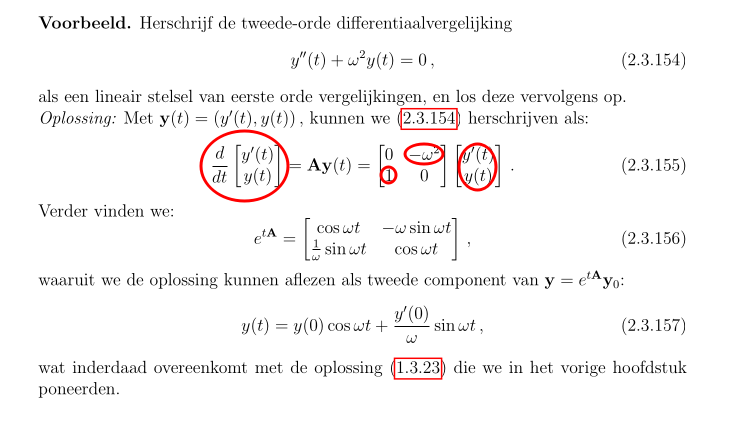
\includegraphics[width=0.95\textwidth]{./images/something.png}
	\end{center}
	\caption{Tweede-orde differentiaalvergelijking}
	\label{fig:diff2}
\end{figure}

\subsection{Symmetrische matrices}

- $A = A^T$
- $A$ heeft enkel reele eigenwaarden
- $A$ heeft orthogonale eigenvectoren
- $A = ODO^T$ met $O$ een orthogonale matrix en $D$ een diagonale matrix

Omdat $O^T = O^{-1}$, kunnen we zeggen dat $O^T O = I$

Ook is het zo dat geometrische multipliciteit = algebraische multipliciteit. -> $A$ is diagonaliseerbaar.

\subsection{SVD (Singular Value Decomposition)}

$A = U \Sigma V^T$

of

$A = \sum_{i=1}^{r} \sigma_i u_i v_i^T$


met $U$ en $V$ orthogonale matrices en $\Sigma$ een diagonale matrix met singular values

$U$ is mxm, $V$ is nxn en $\Sigma$ is mxn


\subsubsection{Example SVD}

Als we compressie willen uitvoeren moeten we essentially SVD uitvoeren, maar onze som wordt beperkt door een rang $r'$

$A = \sum_{i=1}^{r'} \sigma_i u_i v_i^T$

\section*{Formularium}

\subsection*{Taylorontwikkeling}

- $ f(x) = f(a) + f'(a)(x-a) + \frac{f''(a)}{2!}(x-a)^2 + \frac{f'''(a)}{3!}(x-a)^3 + ... $

- $sin(x) = x$ voor kleine $x$

\subsection*{Differentiaalvergelijkingen}

- $y'(x) = \lambda y(x)$

- $y''(x) = \lambda y(x)$ (hier werden 3 gevallen besproken)

\subsection*{Complexe getallen}

- $z = a + bi$ (algemene vorm)

- $i^2 = -1$

- \textbf{inverse}: $(a + bi)^{-1} = \frac{a - bi}{a^2 + b^2}$

- \textbf{complement}: $z = a + bi \rightarrow z^* = a - bi$

- \textbf{modulus}: $|z| = \sqrt{a^2 + b^2}$

- $e^{i\theta} = cos(\theta) + i sin(\theta)$

- $sin^2(x) + cos^2(x) = 1$

- $sin(x) = \frac{e^{ix} - e^{-ix}}{2i}$

- $sin(2x) = 2sin(x)cos(x)$

- $cos(x) = \frac{e^{ix} + e^{-ix}}{2}$

- $cos(2x) = cos^2(x) - sin^2(x)$

\subsection*{Hoofdstelling van de algebra}

$x_1 = \frac{-b + \sqrt{b^2 - 4ac}}{2a}$

$x_2 = \frac{-b - \sqrt{b^2 - 4ac}}{2a}$

met $b = -4*a*c$

\subsection*{Lineare Algebra}

$\frac{u\dot v}{||u|| ||v||} = cos(\theta)$ // Hoek tussen twee vectoren

$v^{||} = (u_1 \dot y) u_1 + (u_2 \dot y) u_2 + ...$ // Projectie van $v$


\section*{Oefeningen}

\subsection*{Huis 1}

\begin{figure}[!htbp]
	\centering
	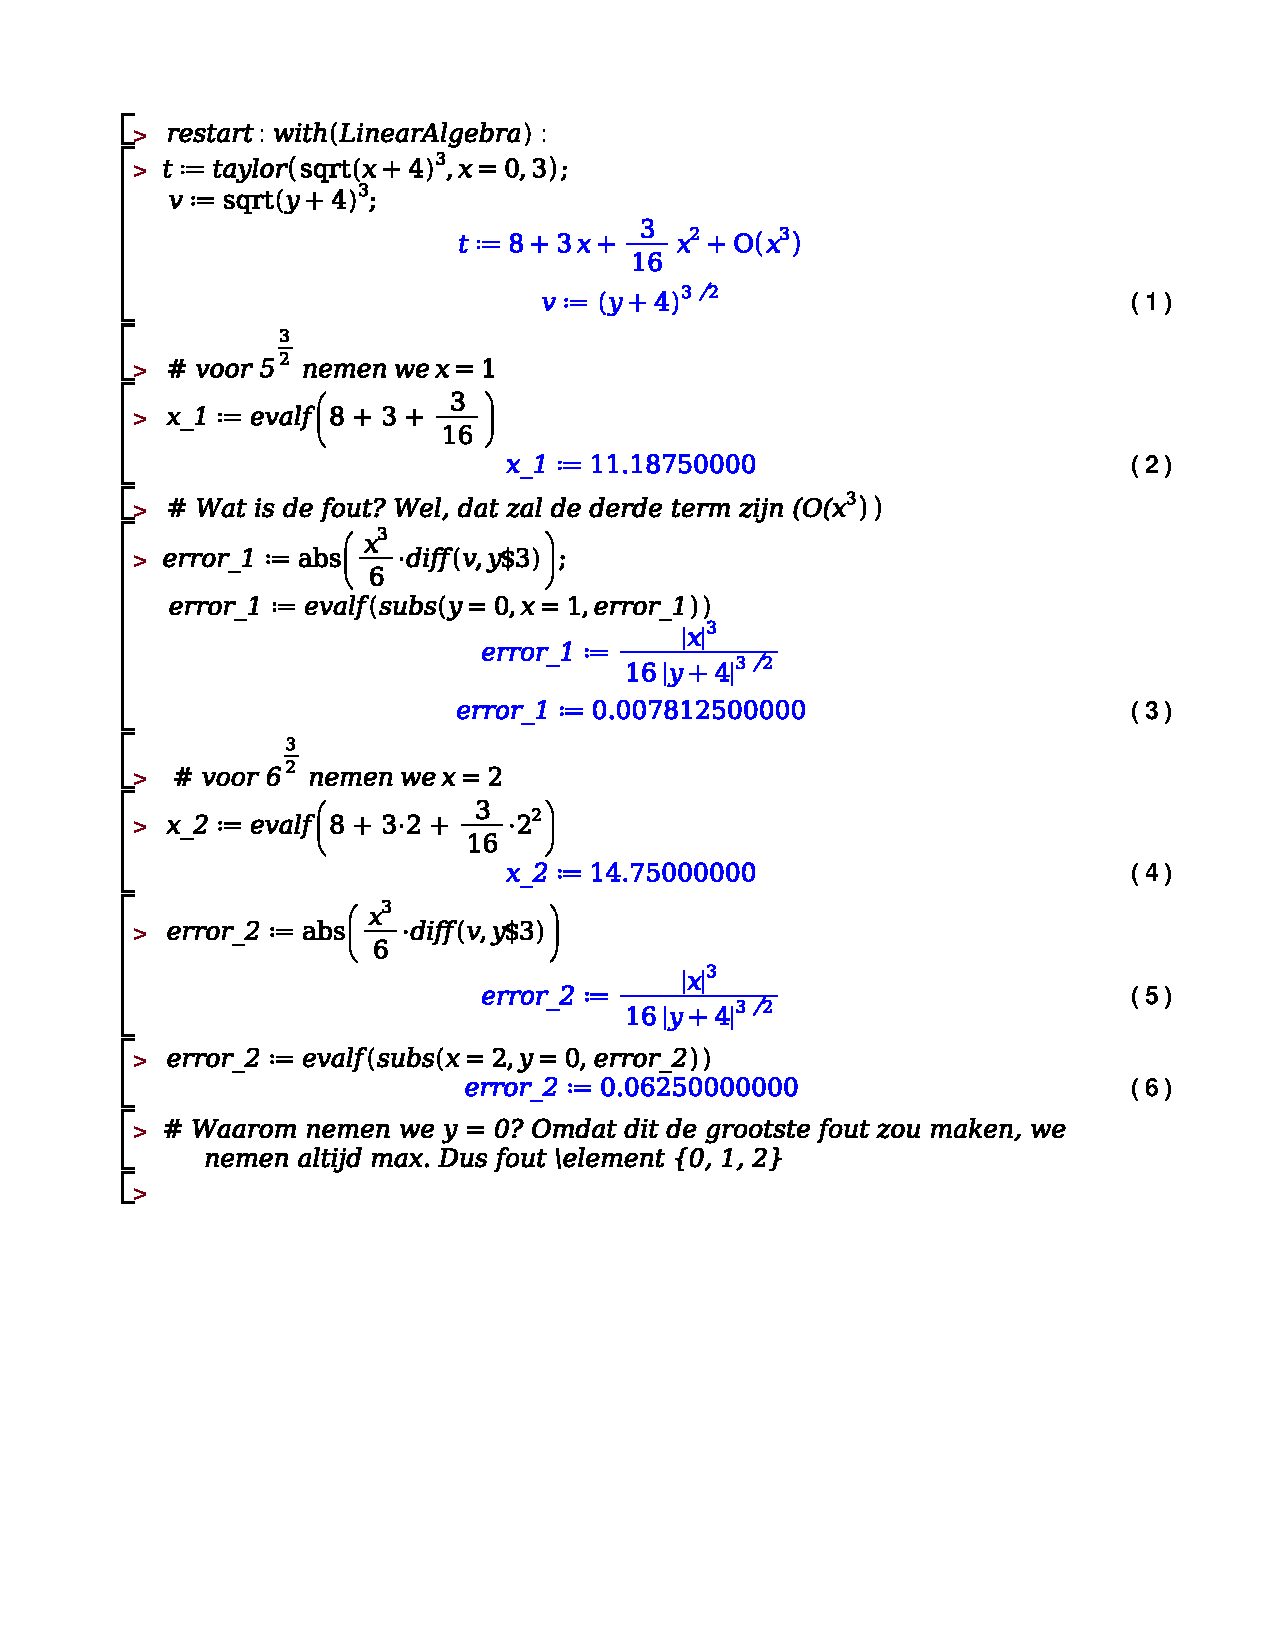
\includegraphics[width=0.8\textwidth]{./exercises/huis_1_ex_1.pdf}
	\caption{Exercise 1}
\end{figure}

\begin{figure}[!htbp]
	\centering
	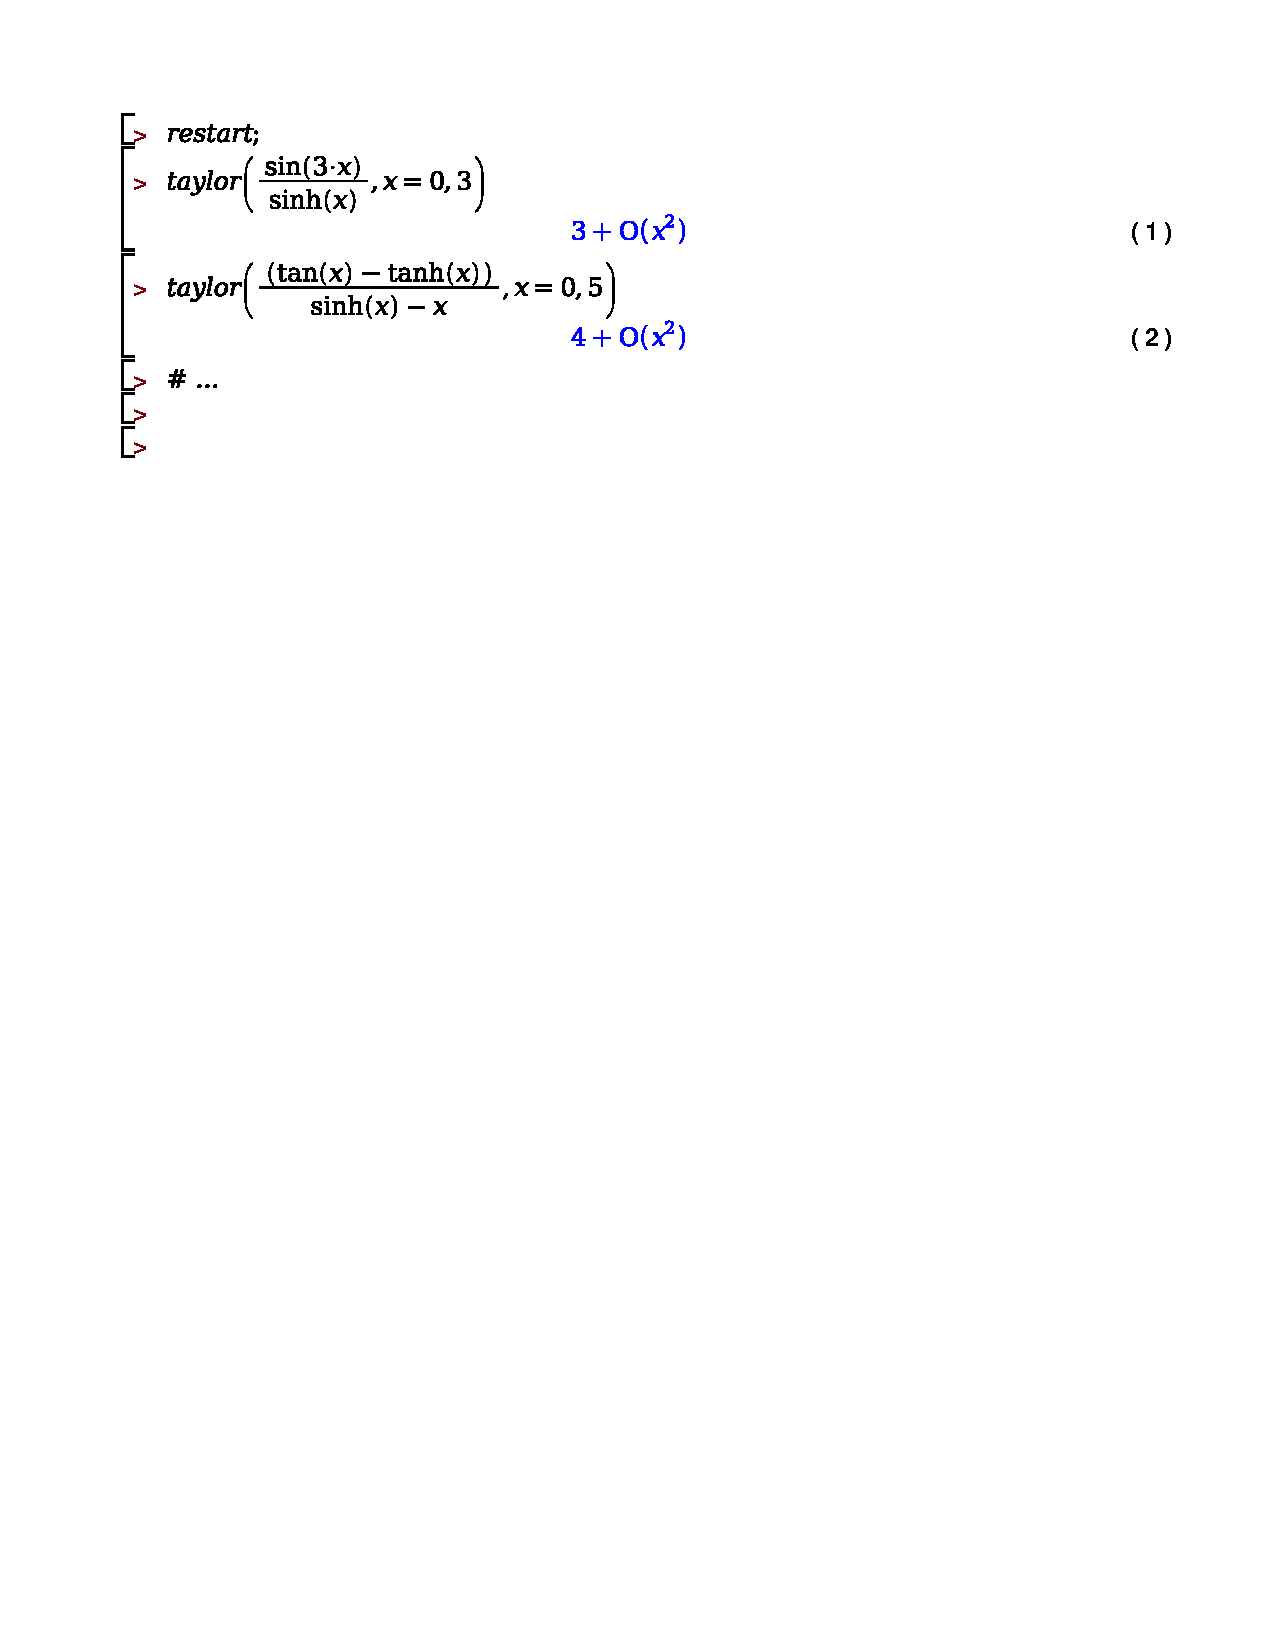
\includegraphics[width=0.8\textwidth]{./exercises/huis_1_ex_2.pdf}
	\caption{Exercise 2}
\end{figure}



\begin{figure}[!htbp]
	\centering
	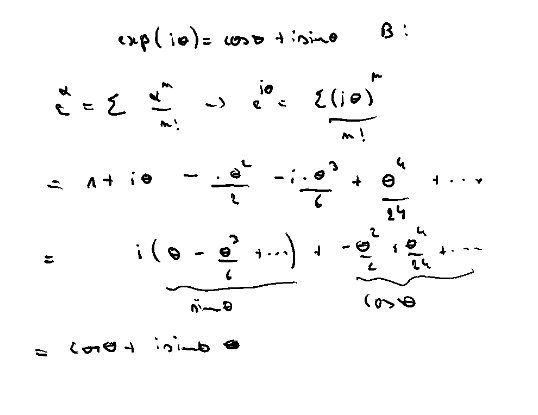
\includegraphics[width=0.8\textwidth]{assets/huis_1_ex_3.png}
	\caption{Exercise 3}
	\label{fig:huis_1_ex_3}
\end{figure}


\begin{figure}[!htbp]
	\centering
	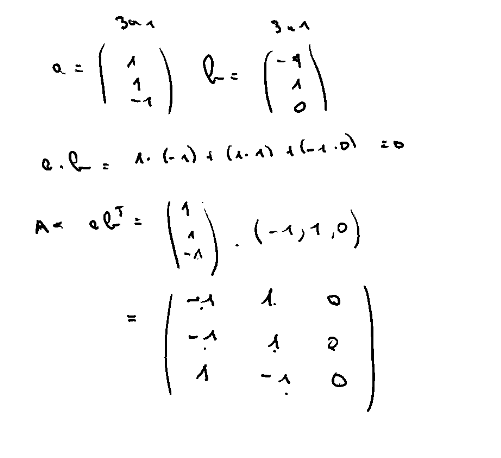
\includegraphics[width=0.6\textwidth]{assets/huis_1_ex_4.png}
	\caption{Exercise 4}
	\label{fig:huis_1_ex_4}
\end{figure}

\newpage

\subsection*{WC 1}

\begin{figure}[!htbp]
	\centering
	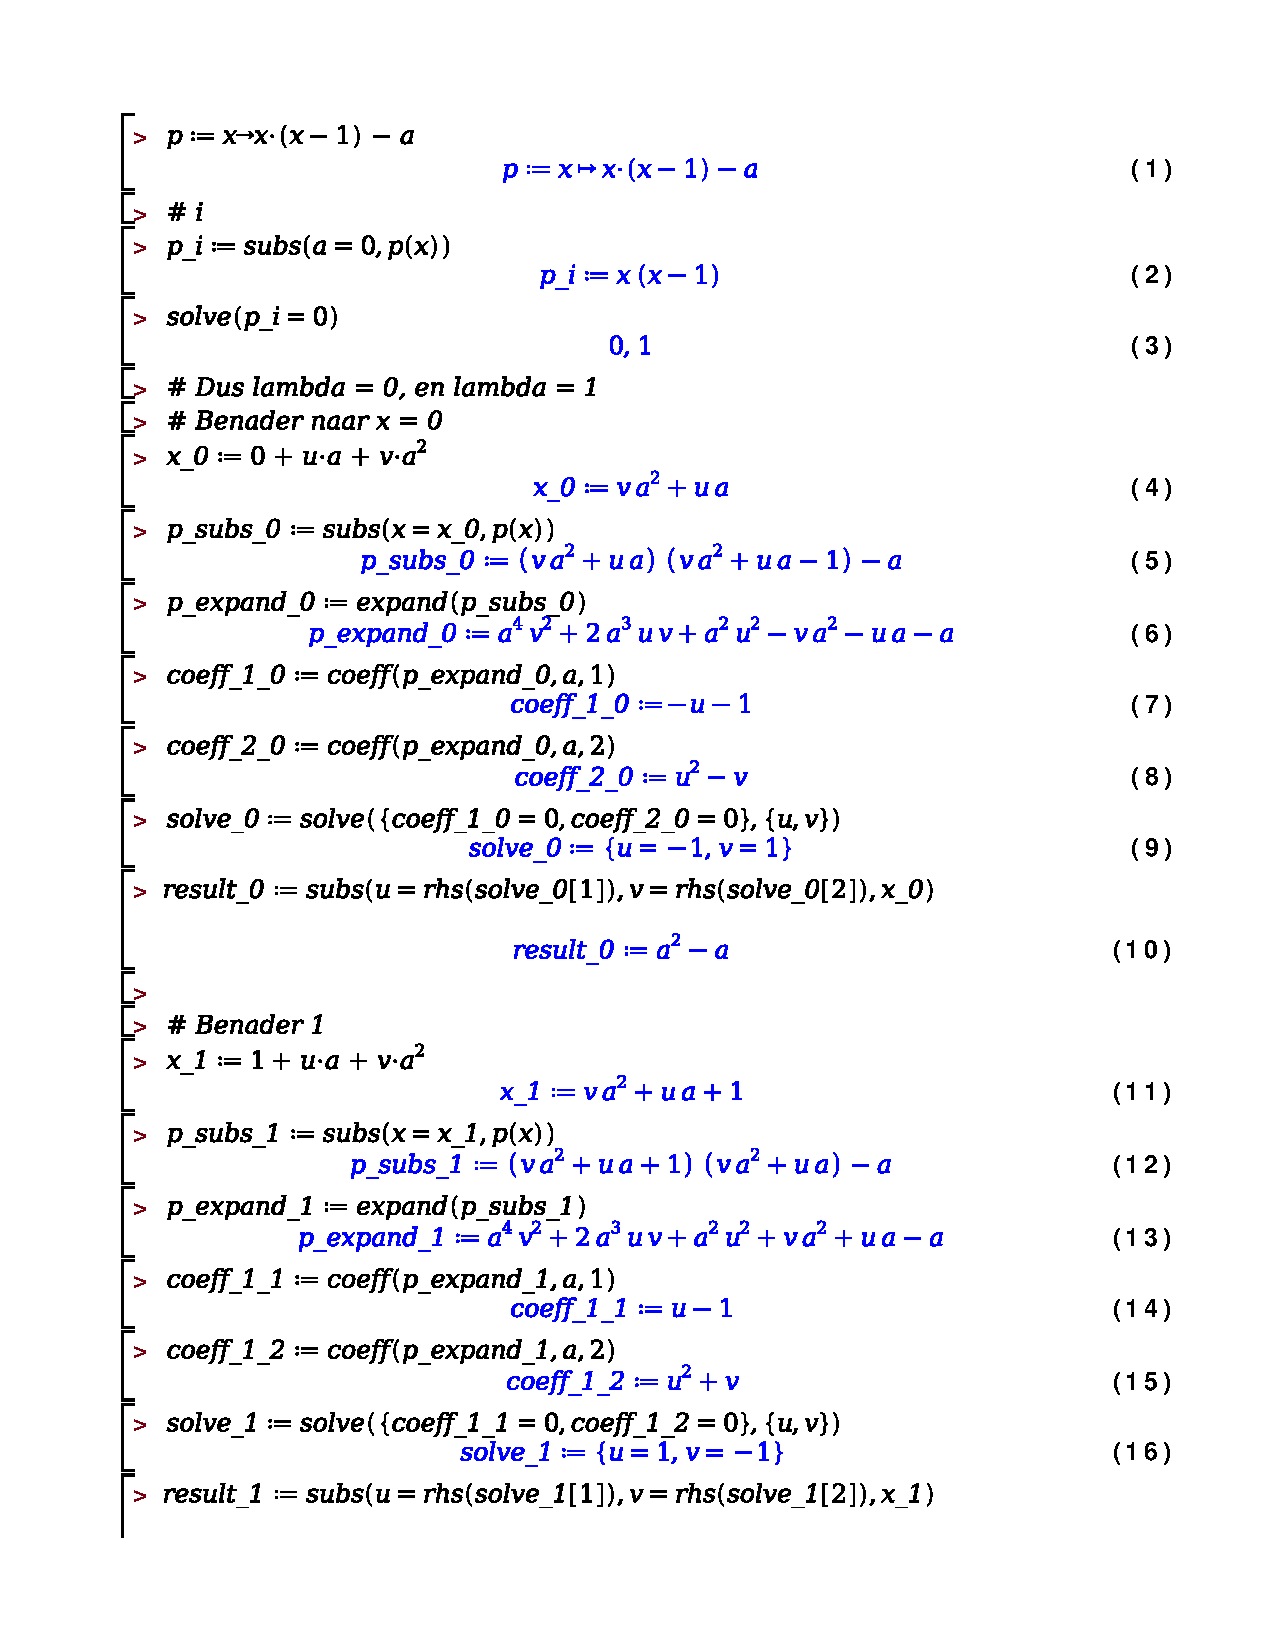
\includegraphics[width=0.8\textwidth]{./exercises/wc_1_ex_1.pdf}
	\caption{Exercise 1}
\end{figure}

\begin{figure}[!htbp]
	\centering
	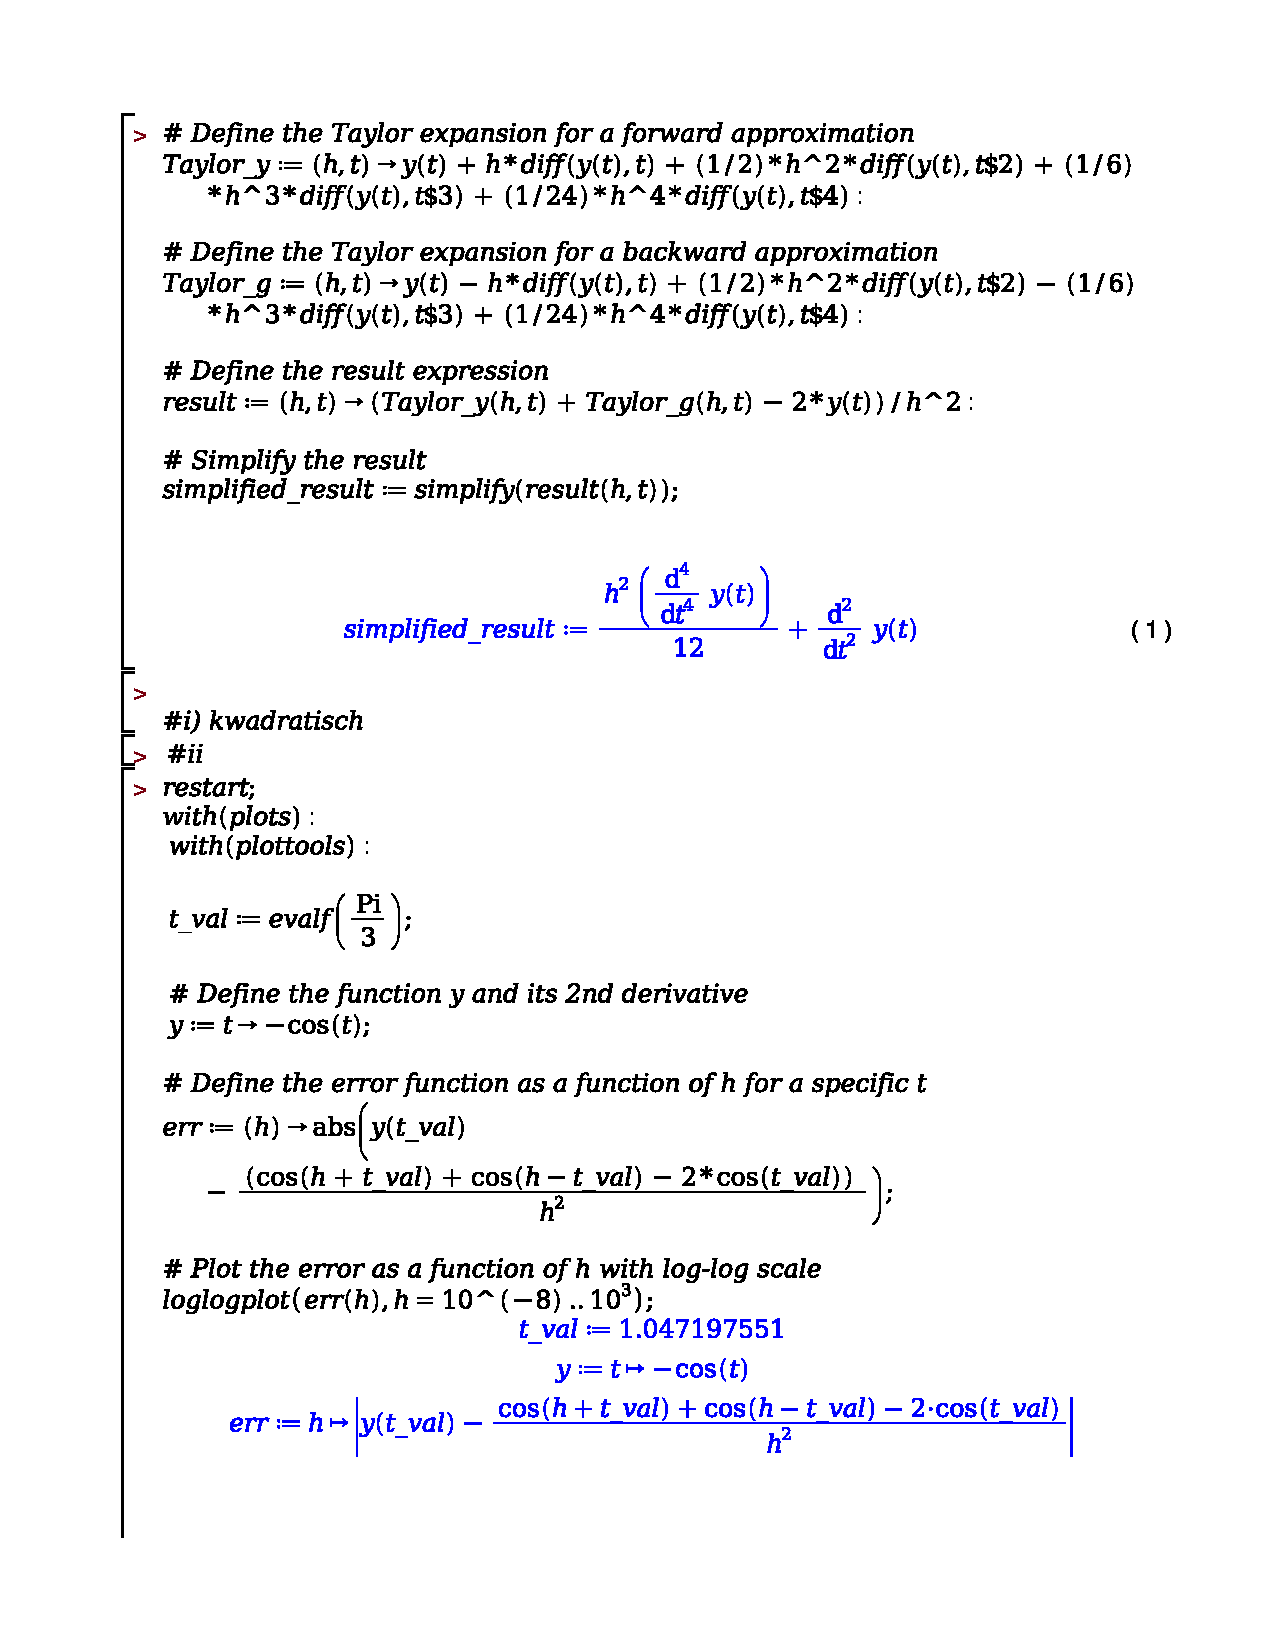
\includegraphics[width=0.8\textwidth]{./exercises/wc_1_ex_2.pdf}
	\caption{Exercise 2}
\end{figure}

\begin{figure}[!htbp]
	\centering
	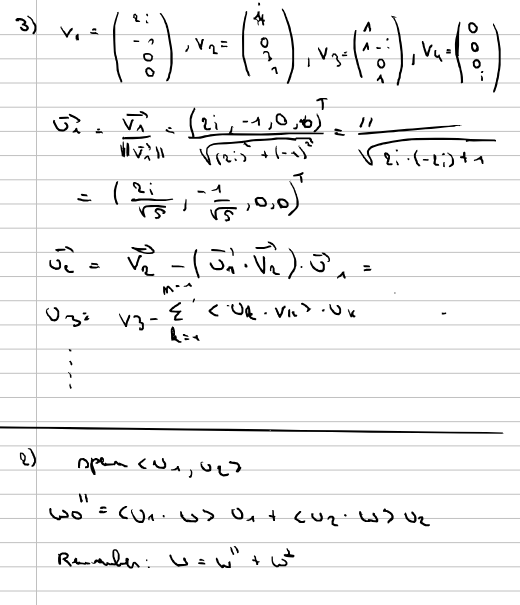
\includegraphics[width=0.8\textwidth]{images/wc1_a3.png}
	\caption{Exercise 3}
\end{figure}

\begin{figure}[!htbp]
	\centering
	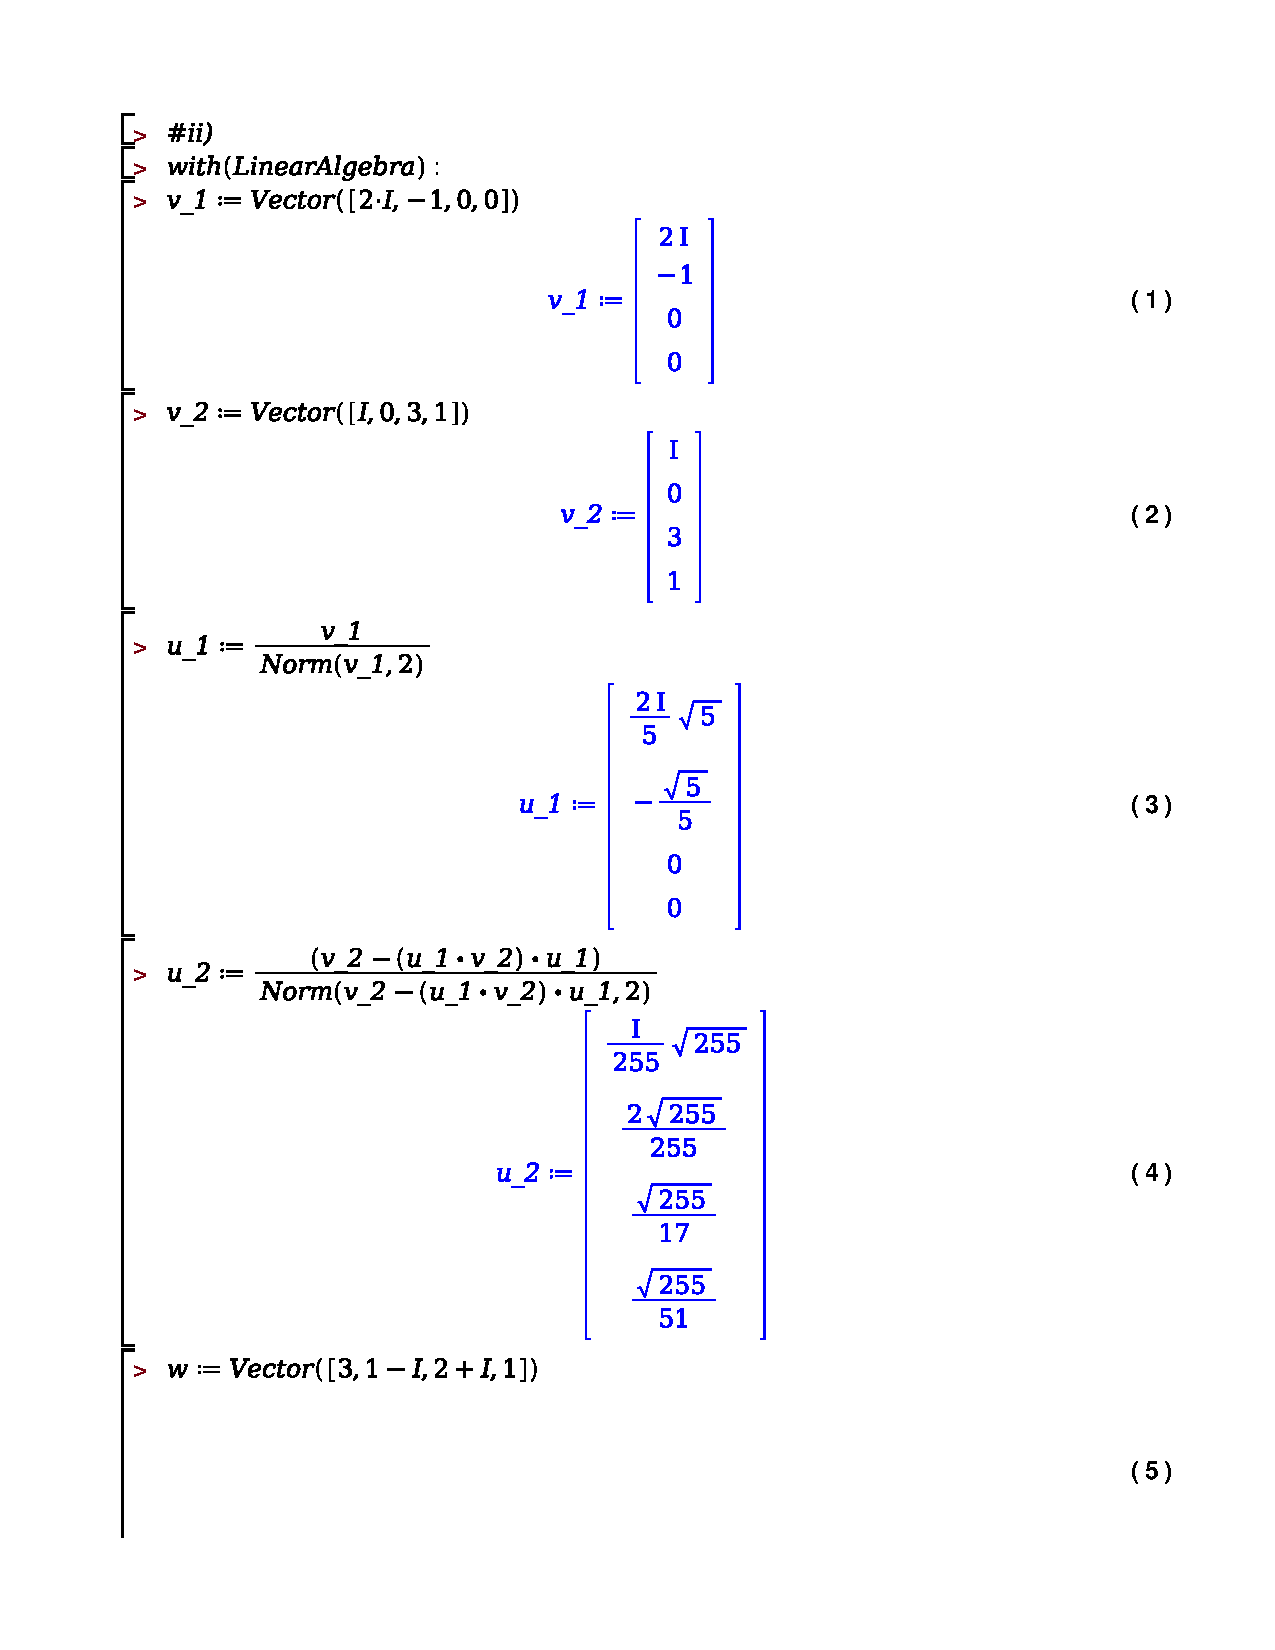
\includegraphics[width=0.8\textwidth]{./exercises/wc_1_ex_3.pdf}
	\caption{Exercise 3}
\end{figure}

\newpage
\subsection*{Bord 1}

\begin{figure}[!htbp]
	\centering
	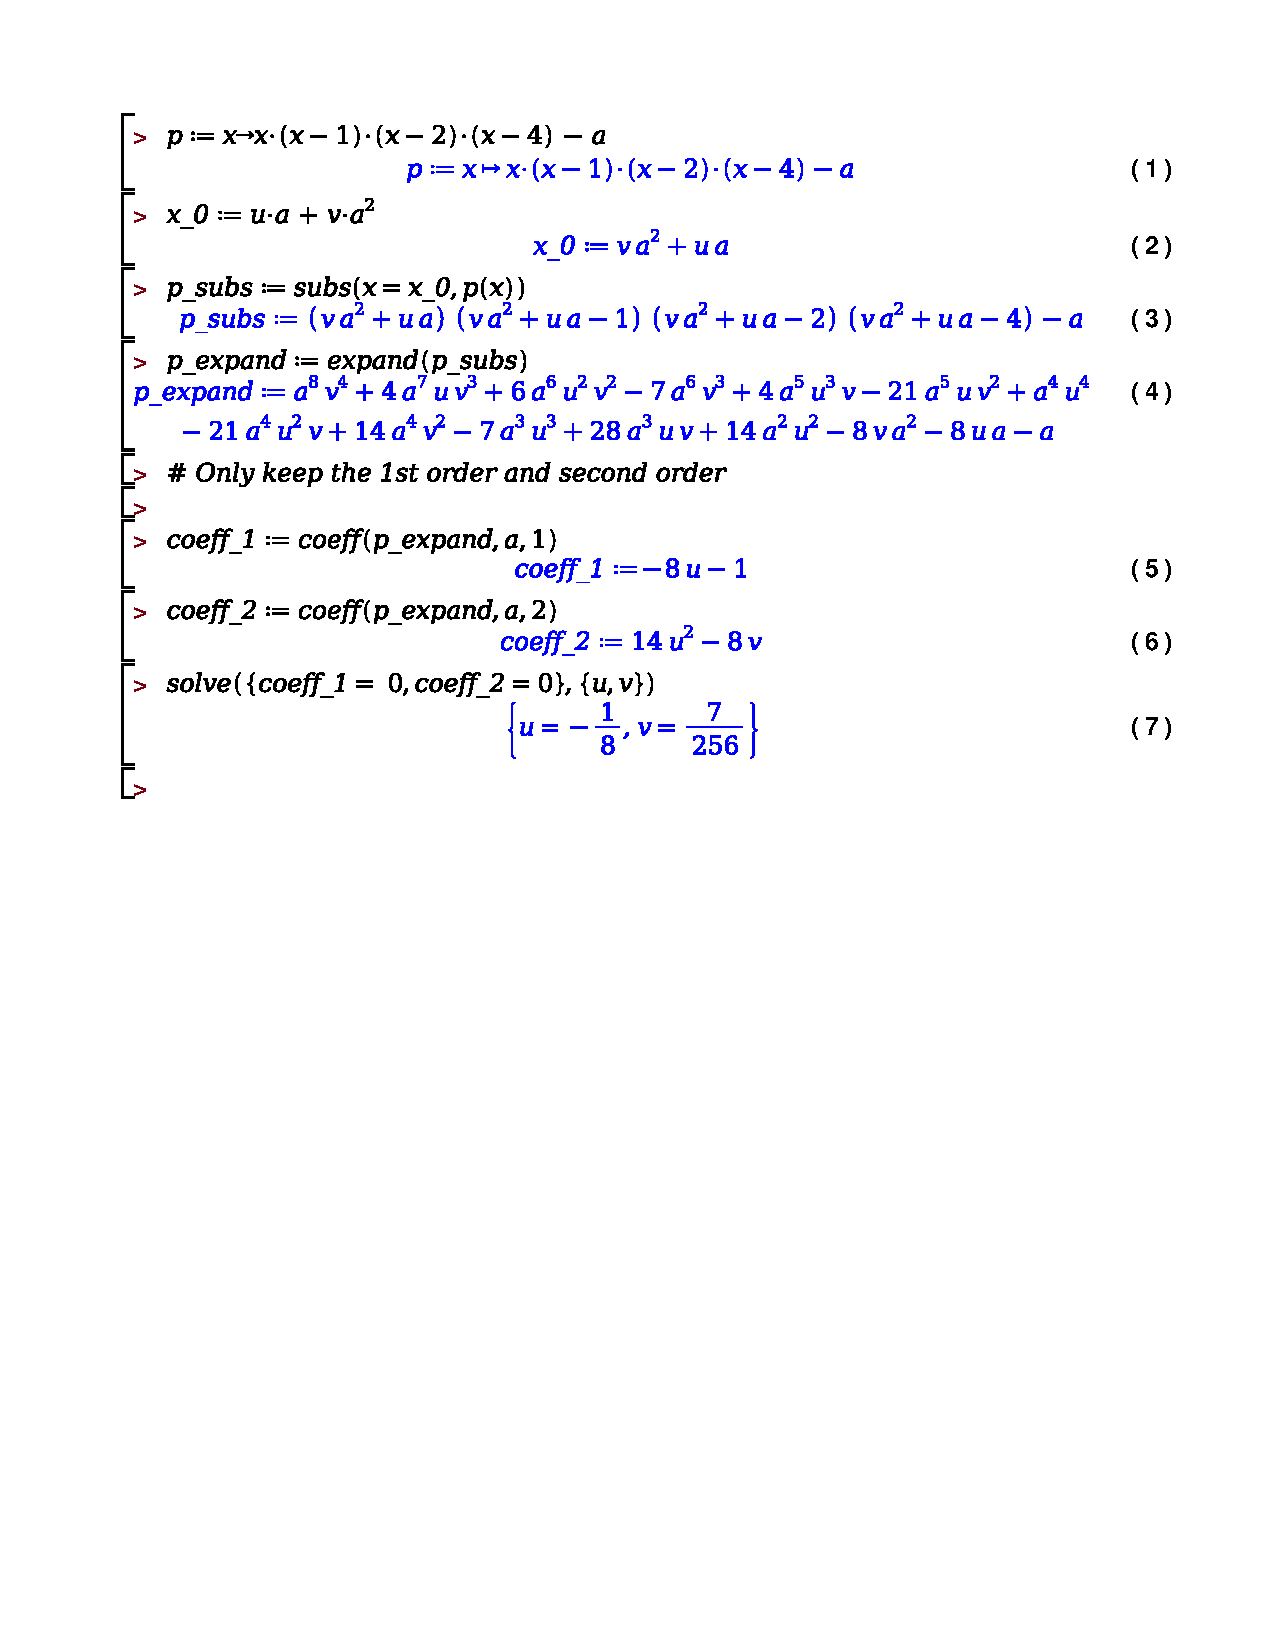
\includegraphics[width=0.8\textwidth]{./exercises/bordles_1.pdf}
	\caption{Exercise 1}
\end{figure}

\begin{figure}[!htbp]
	\centering
	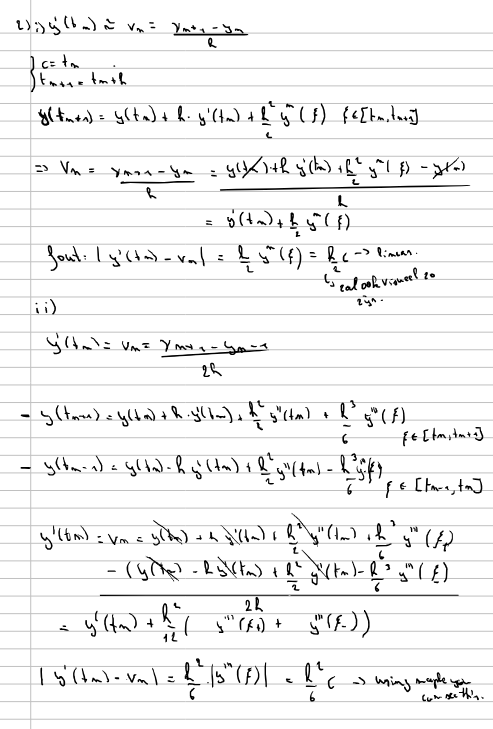
\includegraphics[width=0.8\textwidth]{images/ex_2_a.png}
	\caption{Exercise 2}
\end{figure}

\begin{figure}[!htbp]
	\centering
	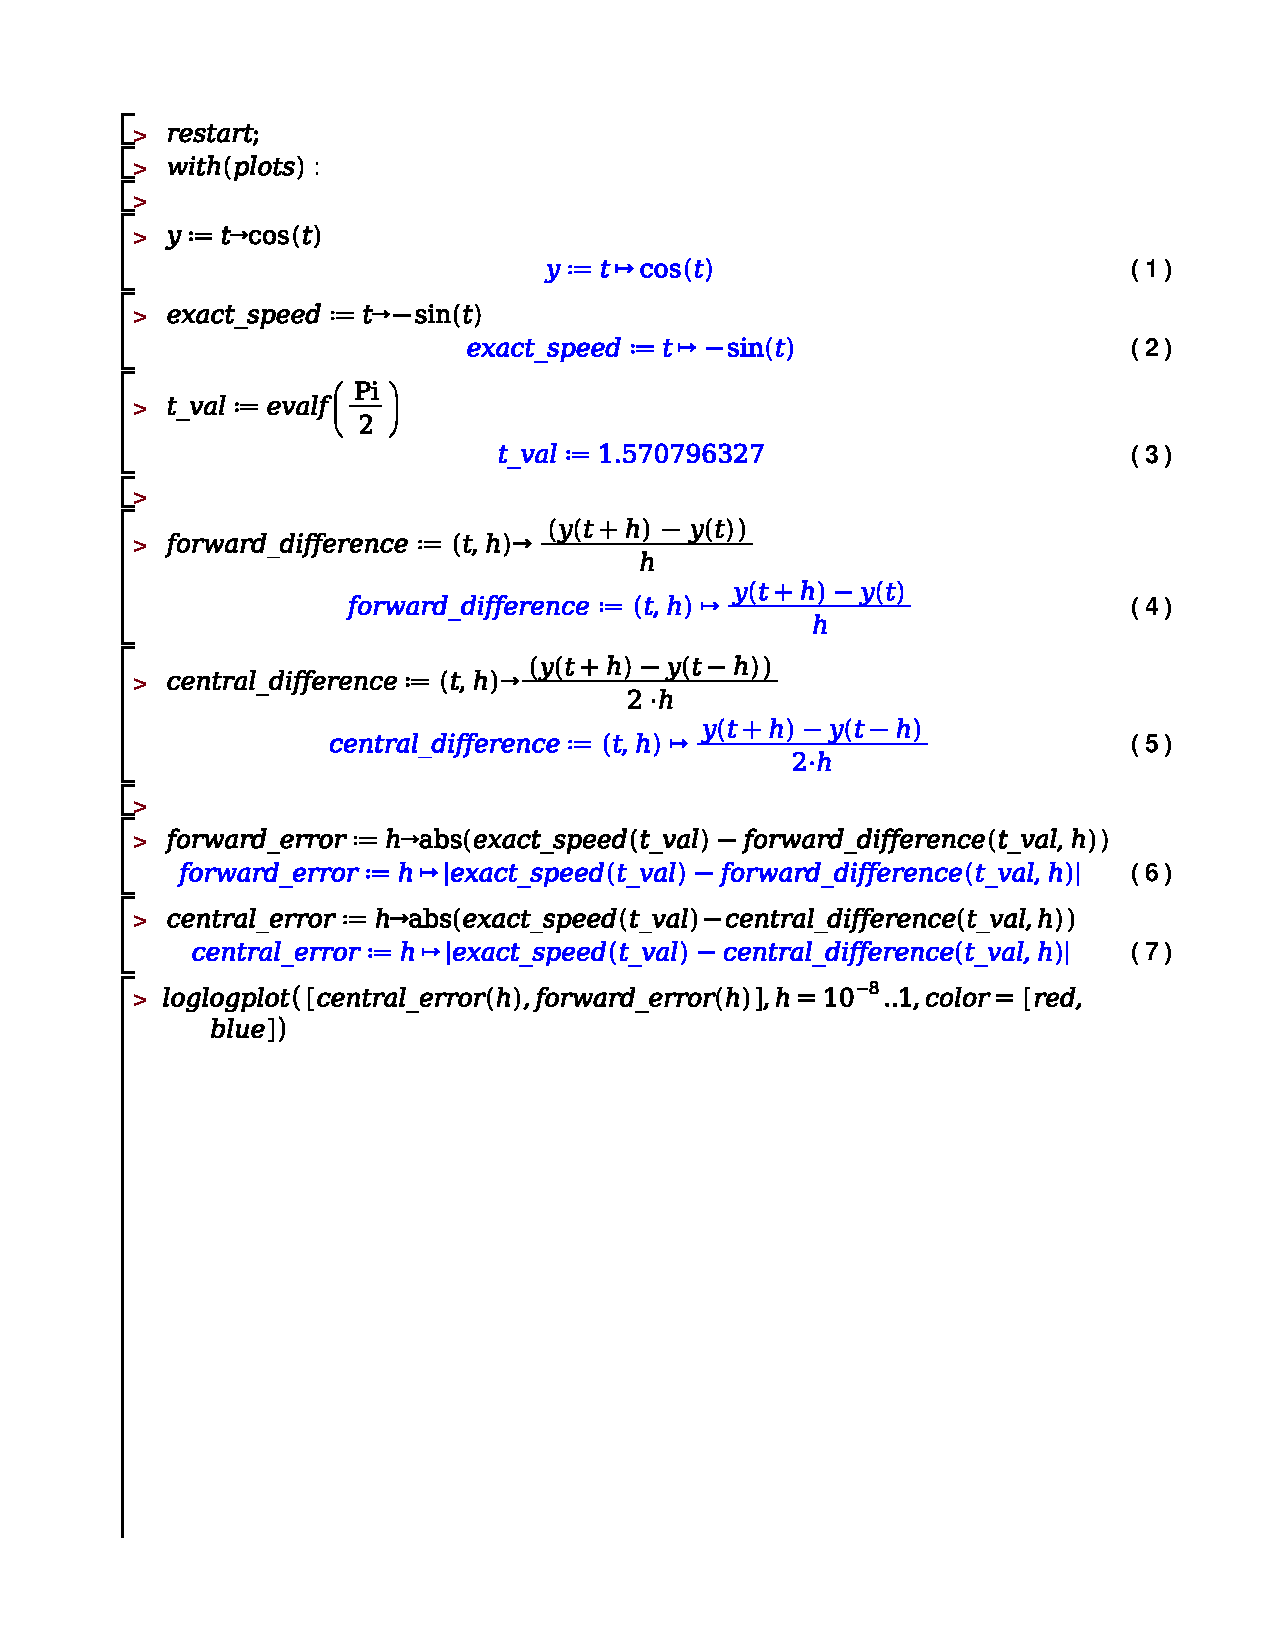
\includegraphics[width=0.8\textwidth]{./exercises/bordles_1_ex_2.pdf}
	\caption{Exercise 2 part 2 Maple}
\end{figure}

\begin{figure}[!htbp]
	\centering
	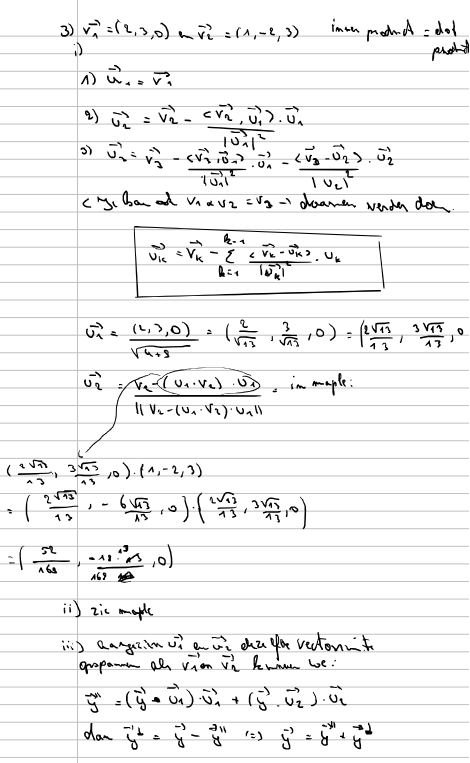
\includegraphics[width=\textwidth]{images/pl_1_answer_3.png}
	\caption{Exercise 3}
\end{figure}

\begin{figure}[!htbp]
	\centering
	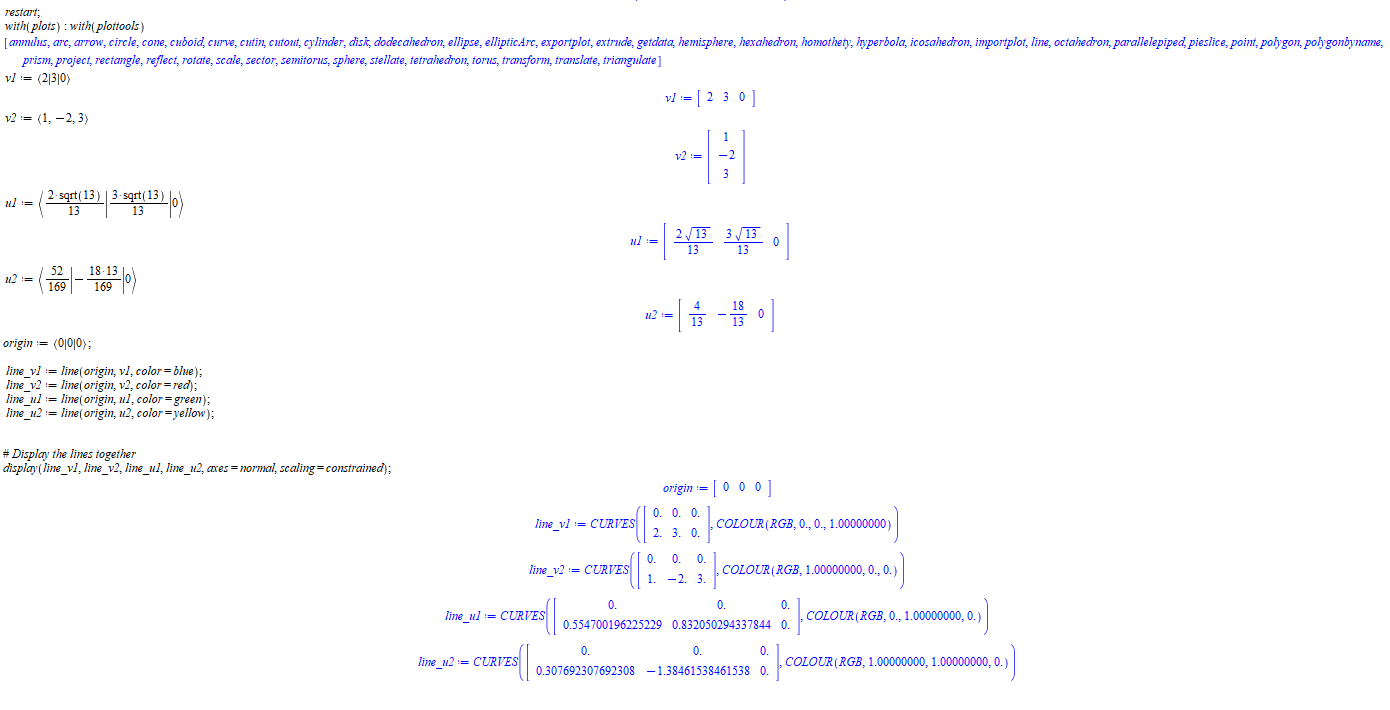
\includegraphics[width=\textwidth]{images/plot_2.png}
	\caption{Exercise 3 - plot }
\end{figure}

\begin{figure}[!htbp]
	\centering
	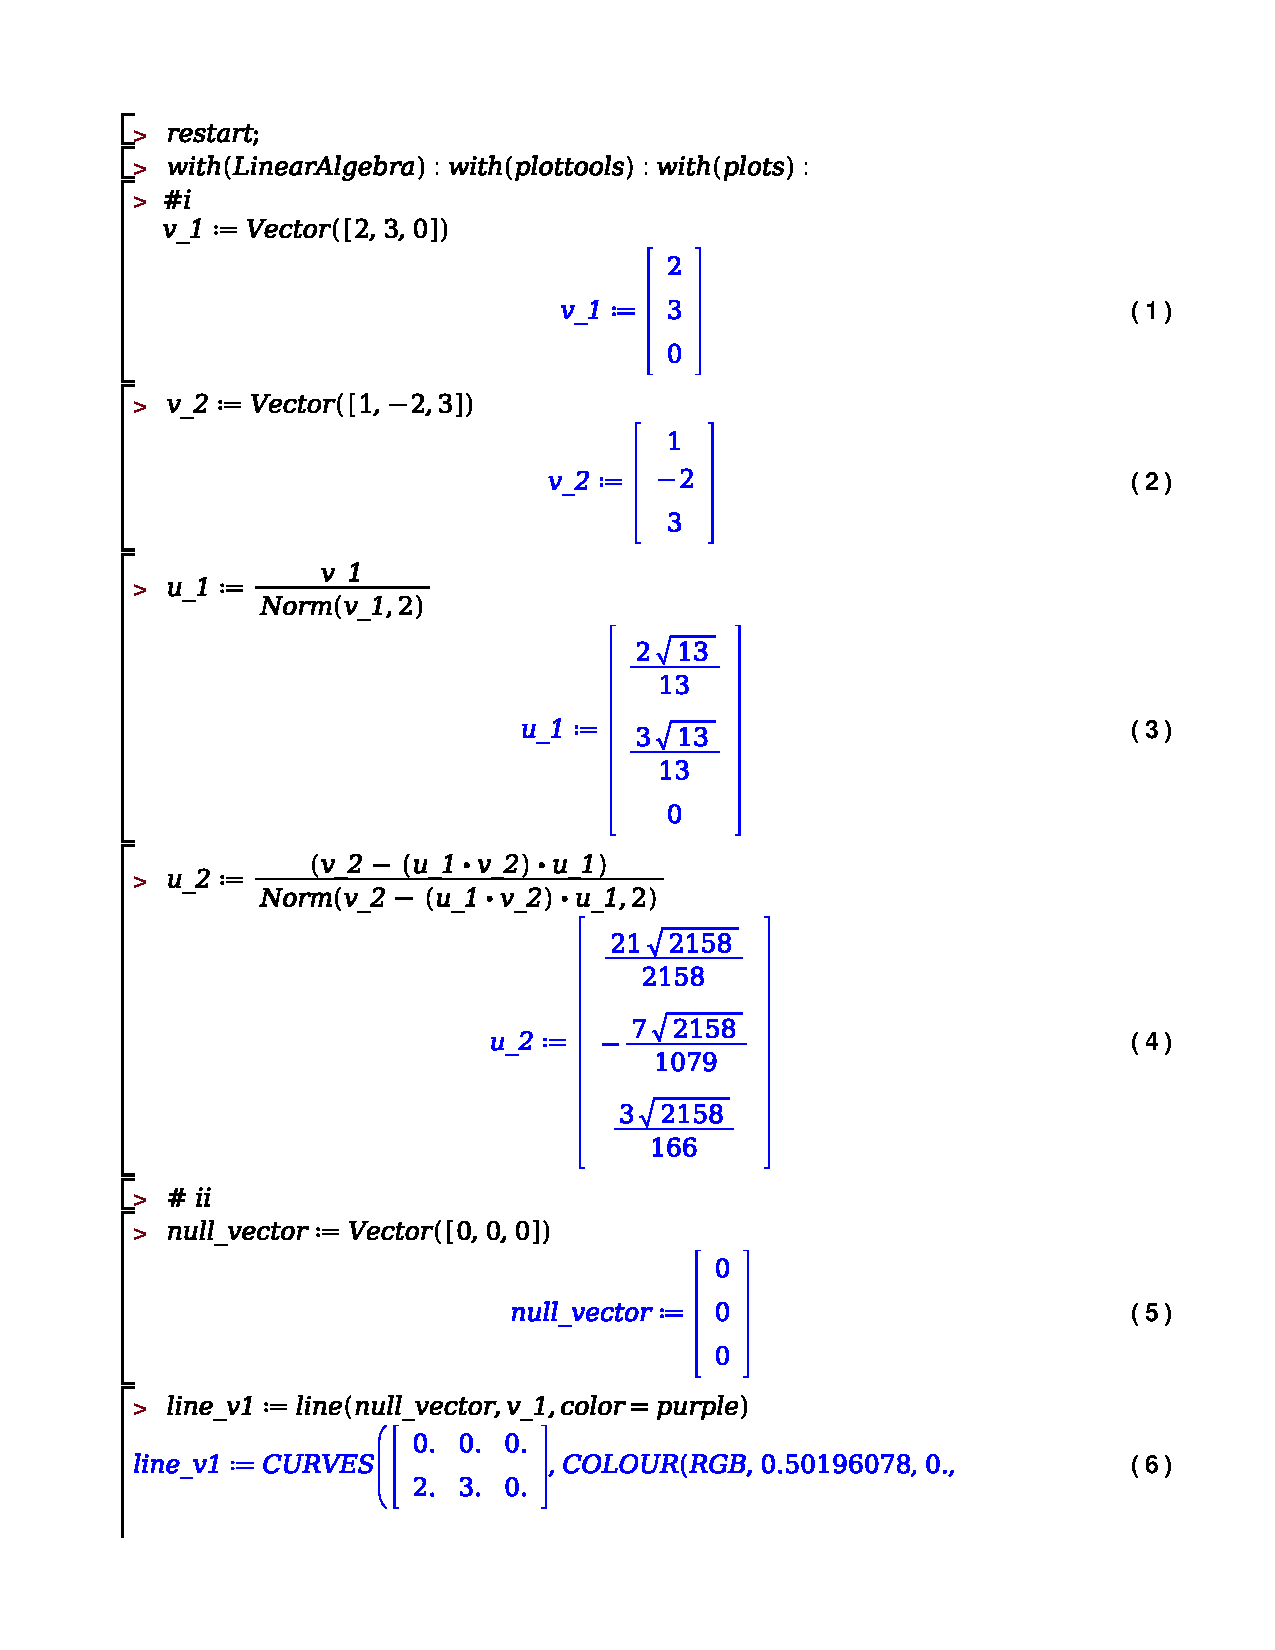
\includegraphics[width=\textwidth]{./exercises/bordles_1_ex_3.pdf}
	\caption{Exercise 3}
\end{figure}







\end{document}

\end{document}
